% Paquets généraux
\documentclass[a4paper,12pt,titlepage]{article}
\usepackage[T1]{fontenc}
\usepackage[utf8]{inputenc}
\usepackage[french]{babel}
\usepackage[gen]{eurosym}
%\usepackage[dvips]{graphicx}
\usepackage{fancyhdr}
\usepackage{pdfpages} 
\usepackage{multido}
\usepackage{hyperref}
%\usepackage{textcomp}
%\usepackage{aeguill}
\usepackage{schemabloc}
\usepackage[bitstream-charter]{mathdesign}

\newcommand{\id}{54}
\newcommand{\nom}{Liaisons mécaniques}
\newcommand{\sequence}{04}
\newcommand{\num}{01}
\newcommand{\type}{TP}
\newcommand{\descrip}{Modélisation d'un solide. Comportement des liaisons mécaniques. Modéliser les mécanismes du laboratoire par un schéma cinématique, paramétré.}
\newcommand{\competences}{A3-C4: Analyse d'architecture et de comportement \\ &  Mod1-C1: Isolement d'un solide ou d'un système de solides \\ &  Mod2-C10-1: Modèle de solide indéformable \\ &  Mod2-C11: Modélisation géométrique et cinématique des mouvements entre solides indéformables \\ &  Mod2-C12: Modélisation cinématique des liaisons entre solides \\ &  Mod2-C15: Modélisation des actions mécaniques \\ &  Rés-C6: Utilisation d'un solveur ou d'un logiciel multi physique \\ &  Com1-C1: Différents descripteurs introduits dans le programme \\ &  Com2-C4: Outils de communication}
\newcommand{\nbcomp}{9}
\newcommand{\systemes}{Plateforme Stewart}
\newcommand{\systemessansaccent}{Plateforme Stewart}
\newcommand{\ilot}{2}
\newcommand{\ilotstr}{02}
\newcommand{\dossierilot}{\detokenize{Ilot_02 Plateforme Stewart}}
\newcommand{\imageun}{Plateforme}

\newcommand{\urlsysteme}{\href{https://www.costadoat.fr/systeme/57}{Ressources système}}
\newcommand{\matlabsimscape}{\href{https://github.com/Costadoat/Sciences-Ingenieur/raw/master/Systemes/Plateforme Stewart/Plateforme_Stewart_Simscape.zip}{Modèle Simscape}}
\newcommand{\solidworks}{\href{https://github.com/Costadoat/Sciences-Ingenieur/raw/master/Systemes/Plateforme Stewart/Plateforme_Stewart_Solidworks.zip}{Modèle Solidworks}}
\newcommand{\edrawings}{\href{https://github.com/Costadoat/Sciences-Ingenieur/raw/master/Systemes/Plateforme Stewart/Plateforme_Stewart.EASM}{Modèle eDrawings}}
\newcommand{\test}{Stewart_param1}
\newcommand{\testi}{Stewart_param2}
\newcommand{\testii}{Stewart_param3}
\newcommand{\testiii}{Stewart_param4}
\newcommand{\testiiii}{Stewart_euler}

\newcommand{\auteurun}{Renaud Costadoat}
\newcommand{\auteurdeux}{Françoise Puig}
\newcommand{\institute}{Lycée Dorian}


\usepackage{color}
\usepackage{xcolor}
\usepackage{colortbl}
\usepackage{helvet}
\renewcommand{\familydefault}{\sfdefault}
\usepackage{amsfonts}
\usepackage{amsmath}
%\usepackage{xspace}
\usepackage{varioref}
\usepackage{tabularx}
%\usepackage{floatflt}
\usepackage{graphics}
\usepackage{wrapfig}
\usepackage{textcomp}
\usepackage{tikz}
\usepackage{wrapfig}
\usepackage{gensymb}
\usepackage[european]{circuitikz}
\usetikzlibrary{babel}
\usepackage{ifthen}
\usepackage{cancel}
\usepackage{etoolbox}
\usepackage{multirow}
%\usepackage{boxedminipage}
\definecolor{gris25}{gray}{0.75}
\definecolor{bleu}{RGB}{18,33,98}
\definecolor{bleuf}{RGB}{42,94,171}
\definecolor{bleuc}{RGB}{231,239,247}
\definecolor{rougef}{RGB}{185,18,27}
\definecolor{rougec}{RGB}{255,188,204}%255,230,231
\definecolor{vertf}{RGB}{103,126,82}
\definecolor{vertc}{RGB}{220,255,191}
\definecolor{forestgreen}{rgb}{0.13,0.54,0.13}
\definecolor{blcr}{rgb}{0.59,0.69,0.84}
\definecolor{blfr}{rgb}{0.32,0.51,0.75}
\definecolor{orfr}{rgb}{0.90,0.42,0.15}
\definecolor{orcr}{rgb}{0.90,0.65,0.50}
\definecolor{orangef}{rgb}{0.659,0.269,0.072}
\definecolor{orange}{rgb}{0.58,0.35,0.063}
\definecolor{orangec}{rgb}{0.43,0.32,0.25}
\definecolor{rcorrect}{rgb}{0.6,0,0}
\definecolor{sequence}{rgb}{0.75,0.75,0.75}
\definecolor{competences}{rgb}{0.61,0.73,0.35}
\definecolor{grisf}{HTML}{222222}
\definecolor{grisc}{HTML}{636363}
\definecolor{normal}{HTML}{4087c4}
\definecolor{info}{HTML}{5bc0de}
\definecolor{success}{RGB}{92,184,92}
\definecolor{warning}{RGB}{240,173,78}
\definecolor{danger}{RGB}{217,83,79}
\hypersetup{                    % parametrage des hyperliens
    colorlinks=true,                % colorise les liens
    breaklinks=true,                % permet les retours à la ligne pour les liens trop longs
    urlcolor= blfr,                 % couleur des hyperliens
    linkcolor= orange,                % couleur des liens internes aux documents (index, figures, tableaux, equations,...)
    citecolor= forestgreen                % couleur des liens vers les references bibliographiques
    }

% Mise en page
\pagestyle{fancy}

\setlength{\hoffset}{-18pt}

\setlength{\oddsidemargin}{0pt} 	% Marge gauche sur pages impaires
\setlength{\evensidemargin}{0pt} 	% Marge gauche sur pages paires
\setlength{\marginparwidth}{00pt} 	% Largeur de note dans la marge
\setlength{\headwidth}{481pt} 	 	% Largeur de la zone de tête (17cm)
\setlength{\textwidth}{481pt} 	 	% Largeur de la zone de texte (17cm)
\setlength{\voffset}{-18pt} 		% Bon pour DOS
\setlength{\marginparsep}{7pt}	 	% Séparation de la marge
\setlength{\topmargin}{-30pt} 		% Pas de marge en haut
\setlength{\headheight}{35pt} 		% Haut de page
\setlength{\headsep}{20pt} 		% Entre le haut de page et le texte
\setlength{\footskip}{30pt} 		% Bas de page + séparation
\setlength{\textheight}{700pt} 		% Hauteur de l'icone zone de texte (25cm)
\setlength\fboxrule{1 pt}
\renewcommand{\baselinestretch}{1}
\setcounter{tocdepth}{1}
\newcommand{\cadre}[2]
{\fbox{
  \begin{minipage}{#1\linewidth}
   \begin{center}
    #2\\
   \end{center}
  \end{minipage}
 }
}

\newcounter{num_quest} \setcounter{num_quest}{0}
\newcounter{num_rep} \setcounter{num_rep}{0}
\newcounter{num_cor} \setcounter{num_cor}{0}

\newcommand{\question}[1]{\refstepcounter{num_quest}\par
~\ \\ \parbox[t][][t]{0.15\linewidth}{\textbf{Question \arabic{num_quest}}}\parbox[t][][t]{0.93\linewidth}{#1}\par
}


\newcommand{\reponse}[1]
{\refstepcounter{num_rep}
\noindent
\rule{\linewidth}{.5pt}
\textbf{Question \arabic{num_rep}:}
\multido{\i=1+1}{#1}{~\ \\}
}

\newcommand{\cor}
{\refstepcounter{num_cor}
\noindent
\rule{\linewidth}{.5pt}
\textbf{Question \arabic{num_cor}:} \\
}

\newcommand{\titre}[1]
{\begin{center}
\cadre{0.8}{\huge #1} 
\end{center}
}


% En tête et pied de page
\fancypagestyle{normal}{%
  \fancyhf{}
\lhead{\nom}
\rhead{
\includegraphics[width=2cm]{../../img/logo}\hspace{2pt}}
\ifdef{\auteurdeux}{\lfoot{\auteurun,\auteurdeux}}{\lfoot{\auteurun}}
\cfoot{Page \thepage}}

\fancypagestyle{correction}{%
  \fancyhf{}
  \lhead{\colorbox{danger}{\begin{minipage}{0.65\paperwidth} \textcolor{white}{\textbf{Correction}} \end{minipage}} }
  \rhead{
\includegraphics[width=2cm]{../../img/logo}}
  \ifdef{\auteurdeux}{\lfoot{\auteurun,\auteurdeux}}{\lfoot{\auteurun}}
  \rfoot{\colorbox{danger}{\begin{minipage}{0.5\paperwidth} \begin{flushright}\textcolor{white}{\textbf{Correction}}\end{flushright} \end{minipage}} }}

\renewcommand{\footrulewidth}{0.4pt}

\usepackage{eso-pic}
\newcommand{\BackgroundPic}{%
\put(0,0){%
\parbox[b][\paperheight]{\paperwidth}{%
\vfill
\begin{center}
\hspace{0.5cm}\vspace{0.5cm}

\includegraphics[width=\paperwidth,height=\paperheight,%
keepaspectratio]{../../img/fond3}%
\end{center}
\vfill
}}}

\newcommand{\BackgroundPicdeux}{%
\put(25,-30){%
\parbox[b][\paperheight]{\paperwidth}{%
\vfill
\begin{center}
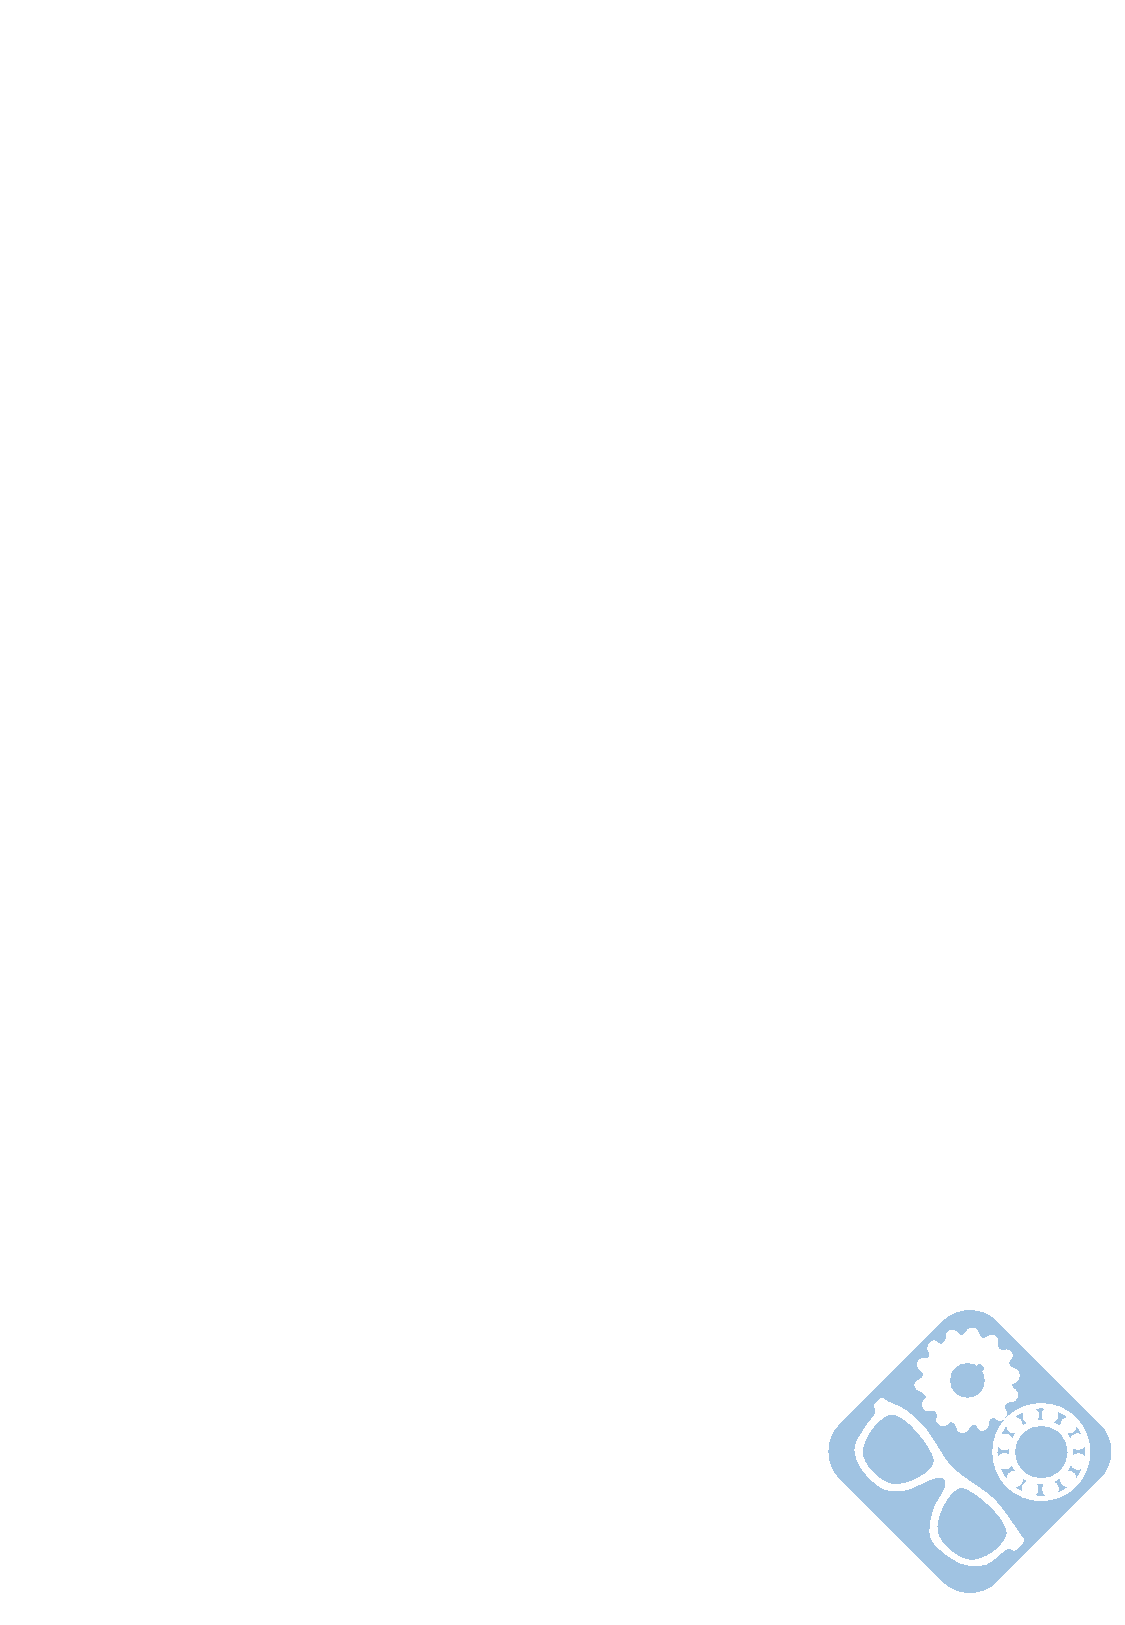
\includegraphics[width=\paperwidth,height=\paperheight,%
keepaspectratio]{../../img/fond4}%
\end{center}
\vfill
}}}

\begin{document}

\pagestyle{empty}

\vspace*{-3\baselineskip}

\AddToShipoutPicture*{\BackgroundPic}

\ifdef{\auteurdeux}{\begin{tabular}{>{\columncolor{gray!00}}m{.3\linewidth} m{.3\linewidth} >{\columncolor{gray!00}}m{.3\linewidth}}
Séquence : \sequence &  \multirow{3}{*}{\hspace{1cm}
\includegraphics[height=1.5cm]{../../img/logo}} &  \begin{flushright} \multirow{4}{*}{\hspace{1cm}
\includegraphics[height=4cm]{img/qrcode}}\end{flushright}\\
Document : \type\num \\
 \institute \\
 \auteurun\\
 \auteurdeux
\end{tabular}}{\begin{tabular}{>{\columncolor{gray!00}}m{.3\linewidth} m{.3\linewidth} >{\columncolor{gray!00}}m{.3\linewidth}}
Séquence : \sequence &  \multirow{3}{*}{\hspace{1cm}
\includegraphics[height=1.5cm]{../../img/logo}} &  \begin{flushright} \multirow{4}{*}{\hspace{1cm}
\includegraphics[height=4cm]{img/qrcode}}\end{flushright}\\
Document : \type\num \\
 \institute \\
 \auteurun
\end{tabular}}

\vspace{1cm}

\ifdef{\prive}{\begin{center}\colorbox{danger}{\Huge{Avec Correction}}\end{center}}{}

\begin{center}\huge{\nom}\end{center}

\vspace{2cm}

\ifdef{\imagedeux}{\begin{minipage}{0.49\linewidth}}{}
\begin{center}\includegraphics[height=5cm]{/home/renaud/Documents/Renaud/GitHub/django_education/systemes/\imageun}\end{center}
\ifdef{\imagedeux}{\end{minipage}\hfill
\begin{minipage}{0.49\linewidth}
\begin{center}\includegraphics[height=5cm]{/home/renaud/Documents/Renaud/GitHub/django_education/systemes/\imagedeux}\end{center}
\end{minipage}}{}

\vspace{5cm}


\begin{tabular}{p{.15\linewidth} >{\columncolor{white}}p{.8\linewidth}}
    \rowcolor{gray!20}
    Référence & S\sequence\ - \type\num \\
    Compétences & \competences \\
 	\rowcolor{gray!20}
    Description & \descrip \\
    Système & \systemes
  \end{tabular}

\newpage

\AddToShipoutPicture{\BackgroundPicdeux}

\pagestyle{normal}

\section{Circuit RC}

\begin{minipage}{0.48\linewidth}
Le composant principal d'un moteur pas à pas est sa bobine. Celle-ci peut être modélisé par une inductance et une résistance propre. Cela se traduit par un circuit RL.

La mise sous tension d'un circuit RL, a donné le relevé temporel suivant.
\end{minipage}\hfill
\begin{minipage}{0.48\linewidth}
\begin{center}
 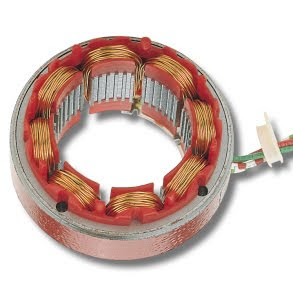
\includegraphics[width=0.7\linewidth]{img/fig1}
\end{center}
\end{minipage}

\begin{center}
 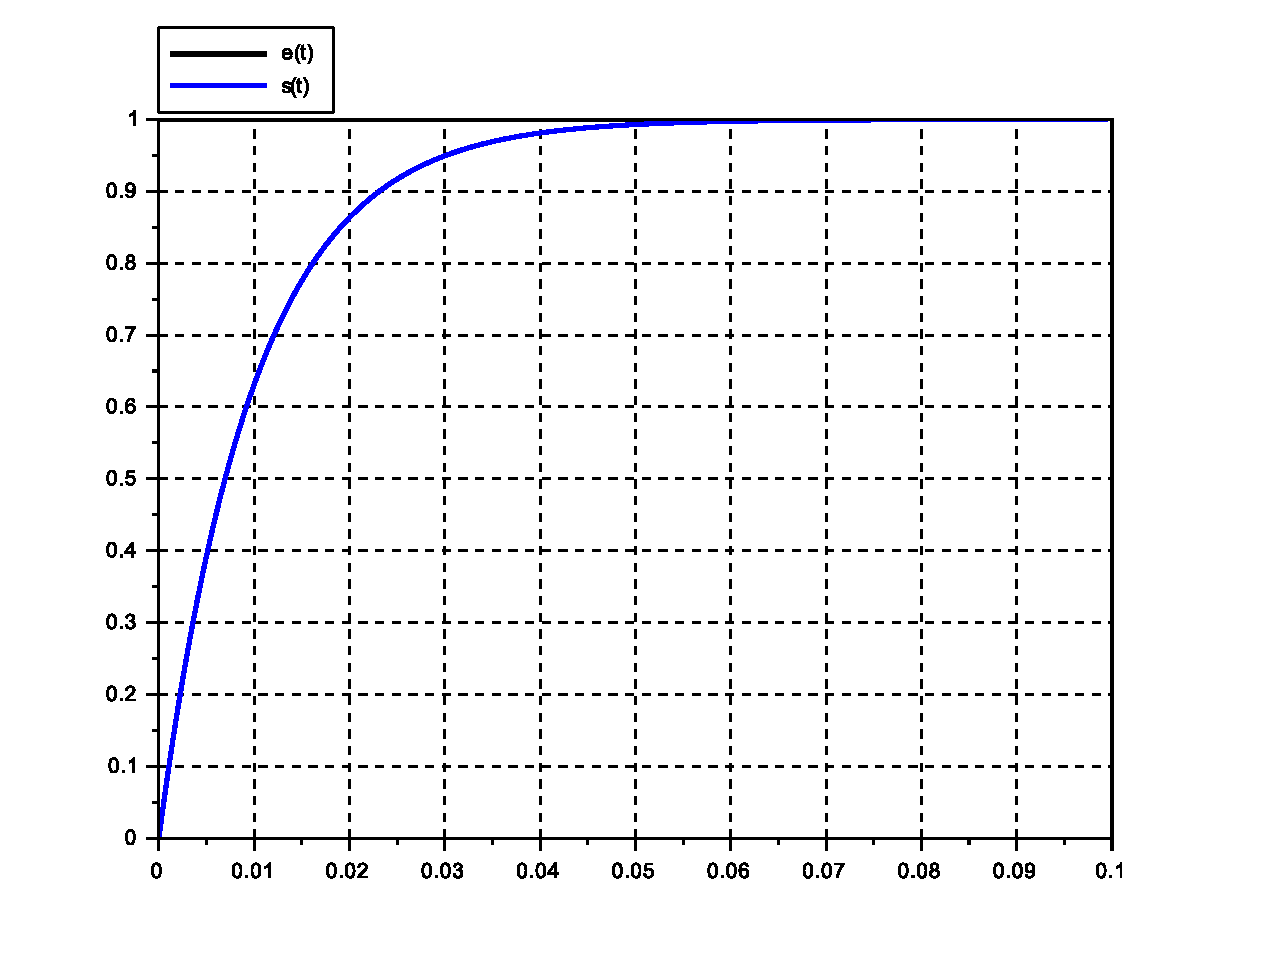
\includegraphics[width=0.7\linewidth]{img/01}
\end{center}

\paragraph{Question 1:} Identifier la fonction de transfert du système en question.

\paragraph{Question 2:} Il est nécessaire d'avoir pour cette application un temps de réponse à 5\% inférieur à 0,06s. Le système respecte-t-il le cahier des charges ?

\newpage

\section{Amortisseur mécanique}


\subsection{Premier réglage}

\begin{minipage}{0.58\linewidth}
La suspension d'une moto est un organe primordial qui permet d'assurer la stabilité du pilote. Il est composé d'un amortisseur et d'un ressort.

L'étude de l'application d'un choc sur une fourche de moto, ayant un réglage 1, a donné les relevés temporel et fréquentiel suivants. L'entrée étant, pour la réponse temporelle, une impulsion en effort de 10N, le graphe suivant affiche le déplacement de la fourche en mètre.

\begin{center}
 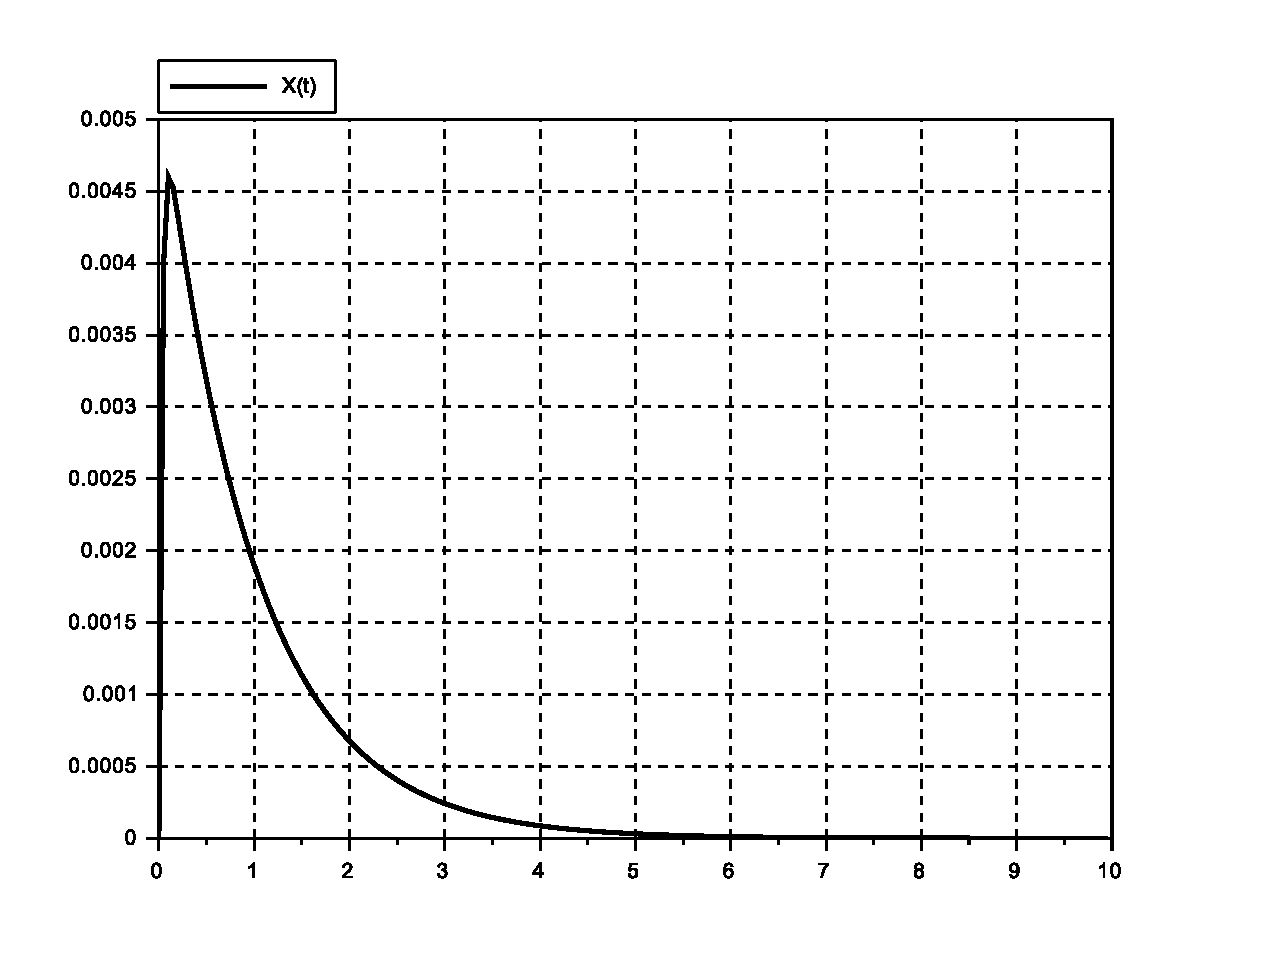
\includegraphics[width=\linewidth]{img/02}
\end{center}

\end{minipage}\hfill
\begin{minipage}{0.38\linewidth}
\begin{center}
 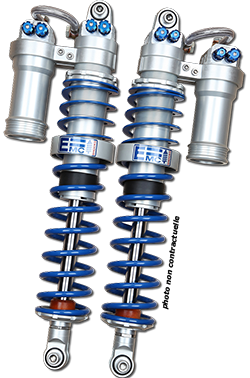
\includegraphics[width=0.7\linewidth]{img/fig2}
\end{center}
\end{minipage}

\begin{center}
 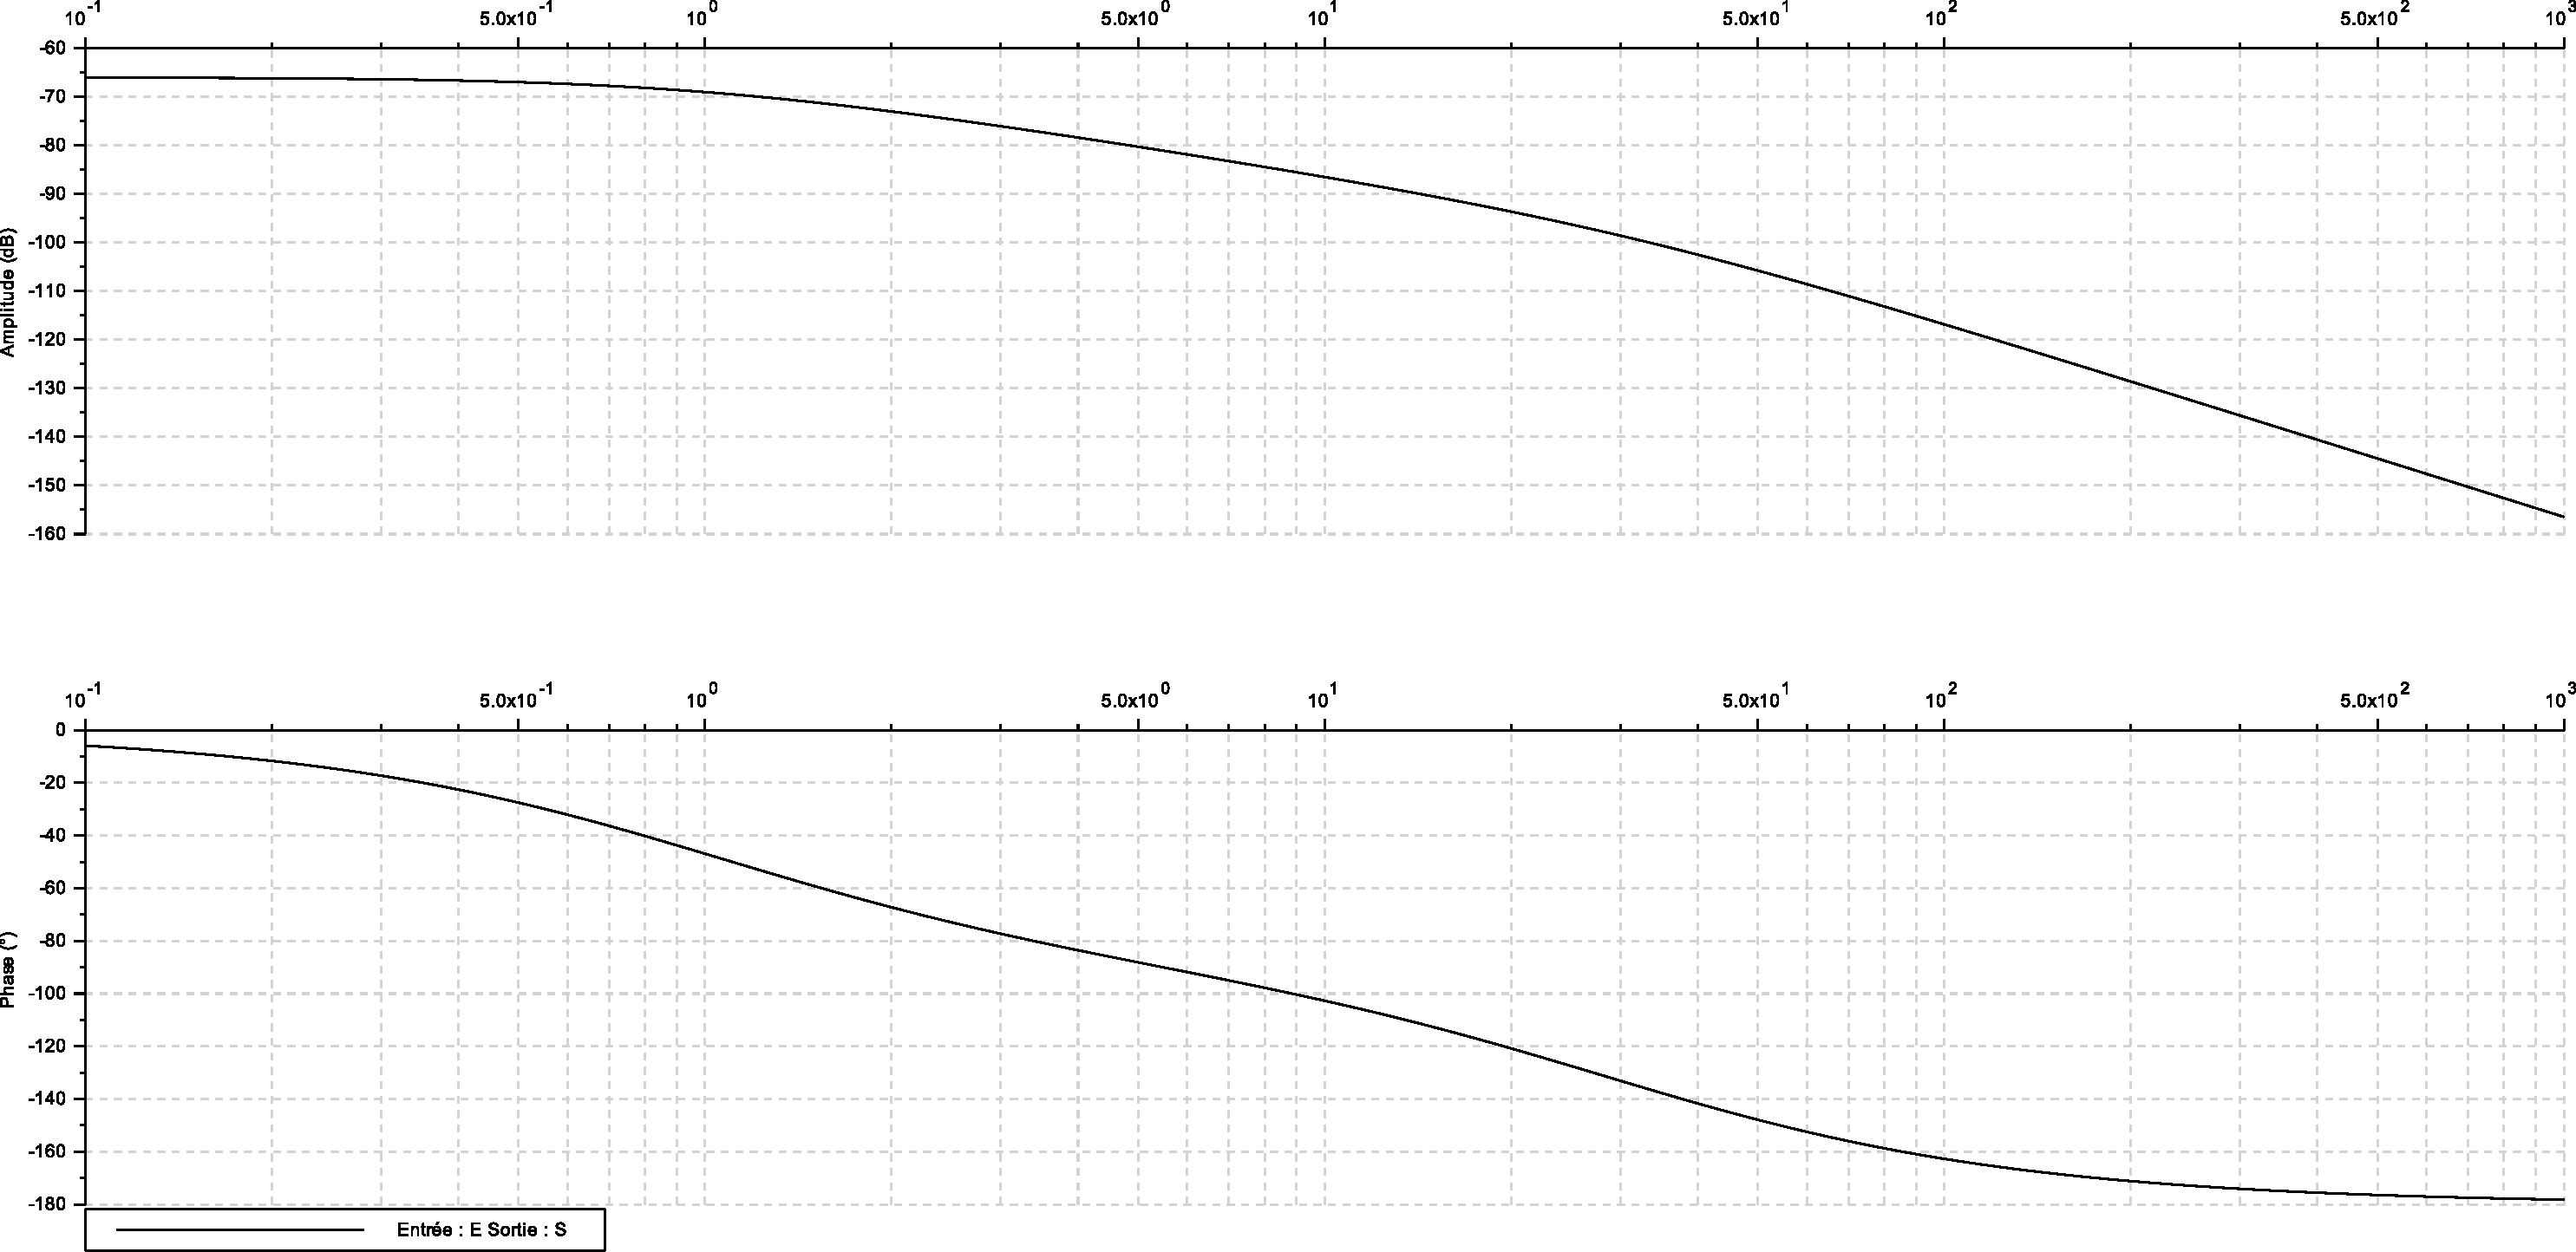
\includegraphics[width=0.9\linewidth]{img/02b}
\end{center}

\paragraph{Question 1:} Identifier la fonction de transfert du système en question.

\paragraph{Question 2:} Il est nécessaire afin de ne pas subir de chocs trop important d'avoir un déplacement de 15cm, lors d'un choc de 100N sur la roue de la moto. Le système dans son état actuel répond-il à cette exigence ?

\subsection{Deuxième réglage}

Un nouveau réglage est proposé pour l'amortissement de la moto, il est présenté dans les relevés temporel et fréquentiel suivants. Dans ce cas, le relevé temporel est un déplacement en mètre en réponse à un échelon de force de 10N.

\begin{center}
 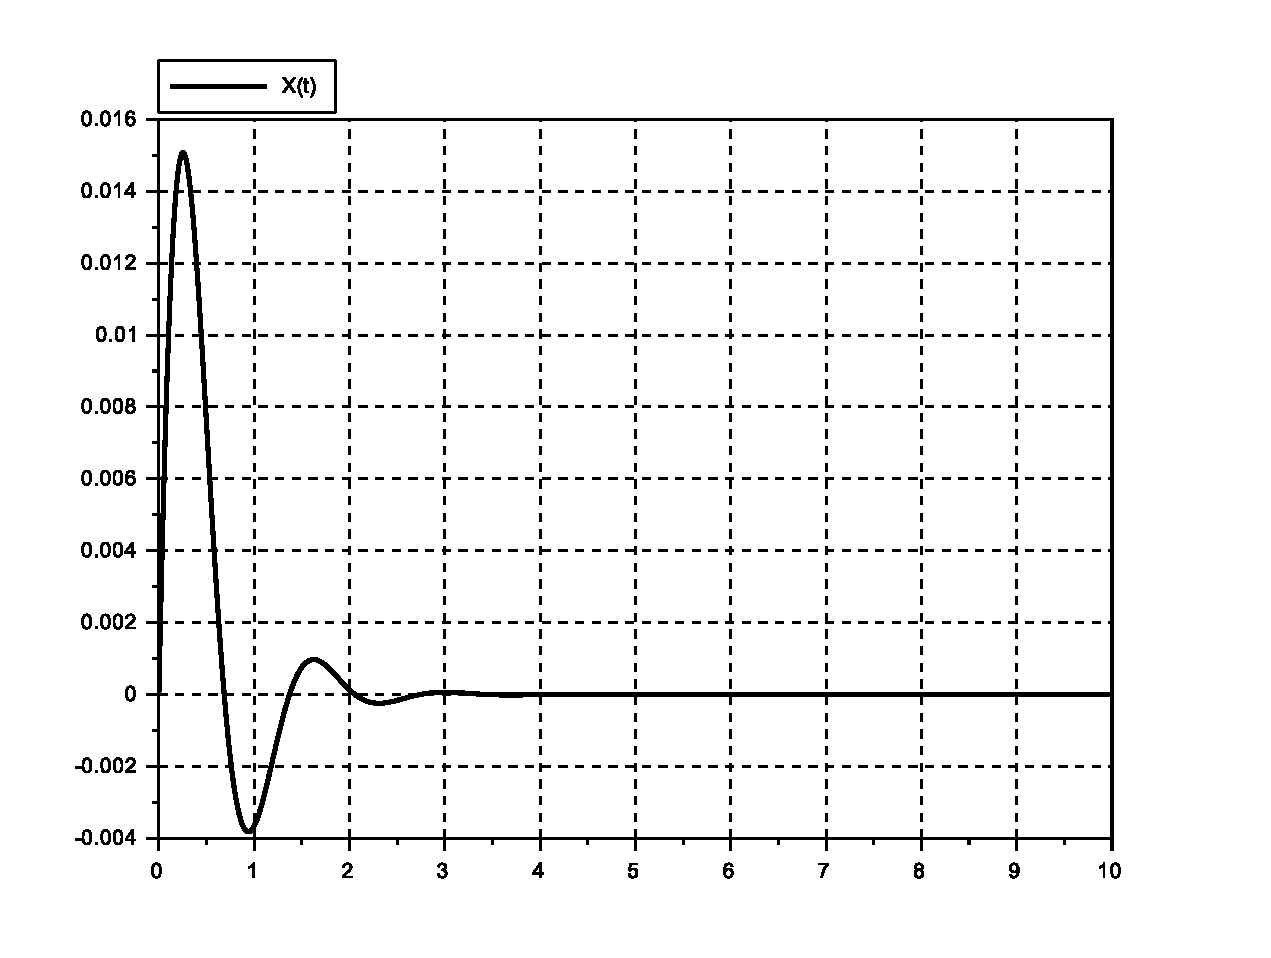
\includegraphics[width=0.65\linewidth]{img/03}
\end{center}

\begin{center}
 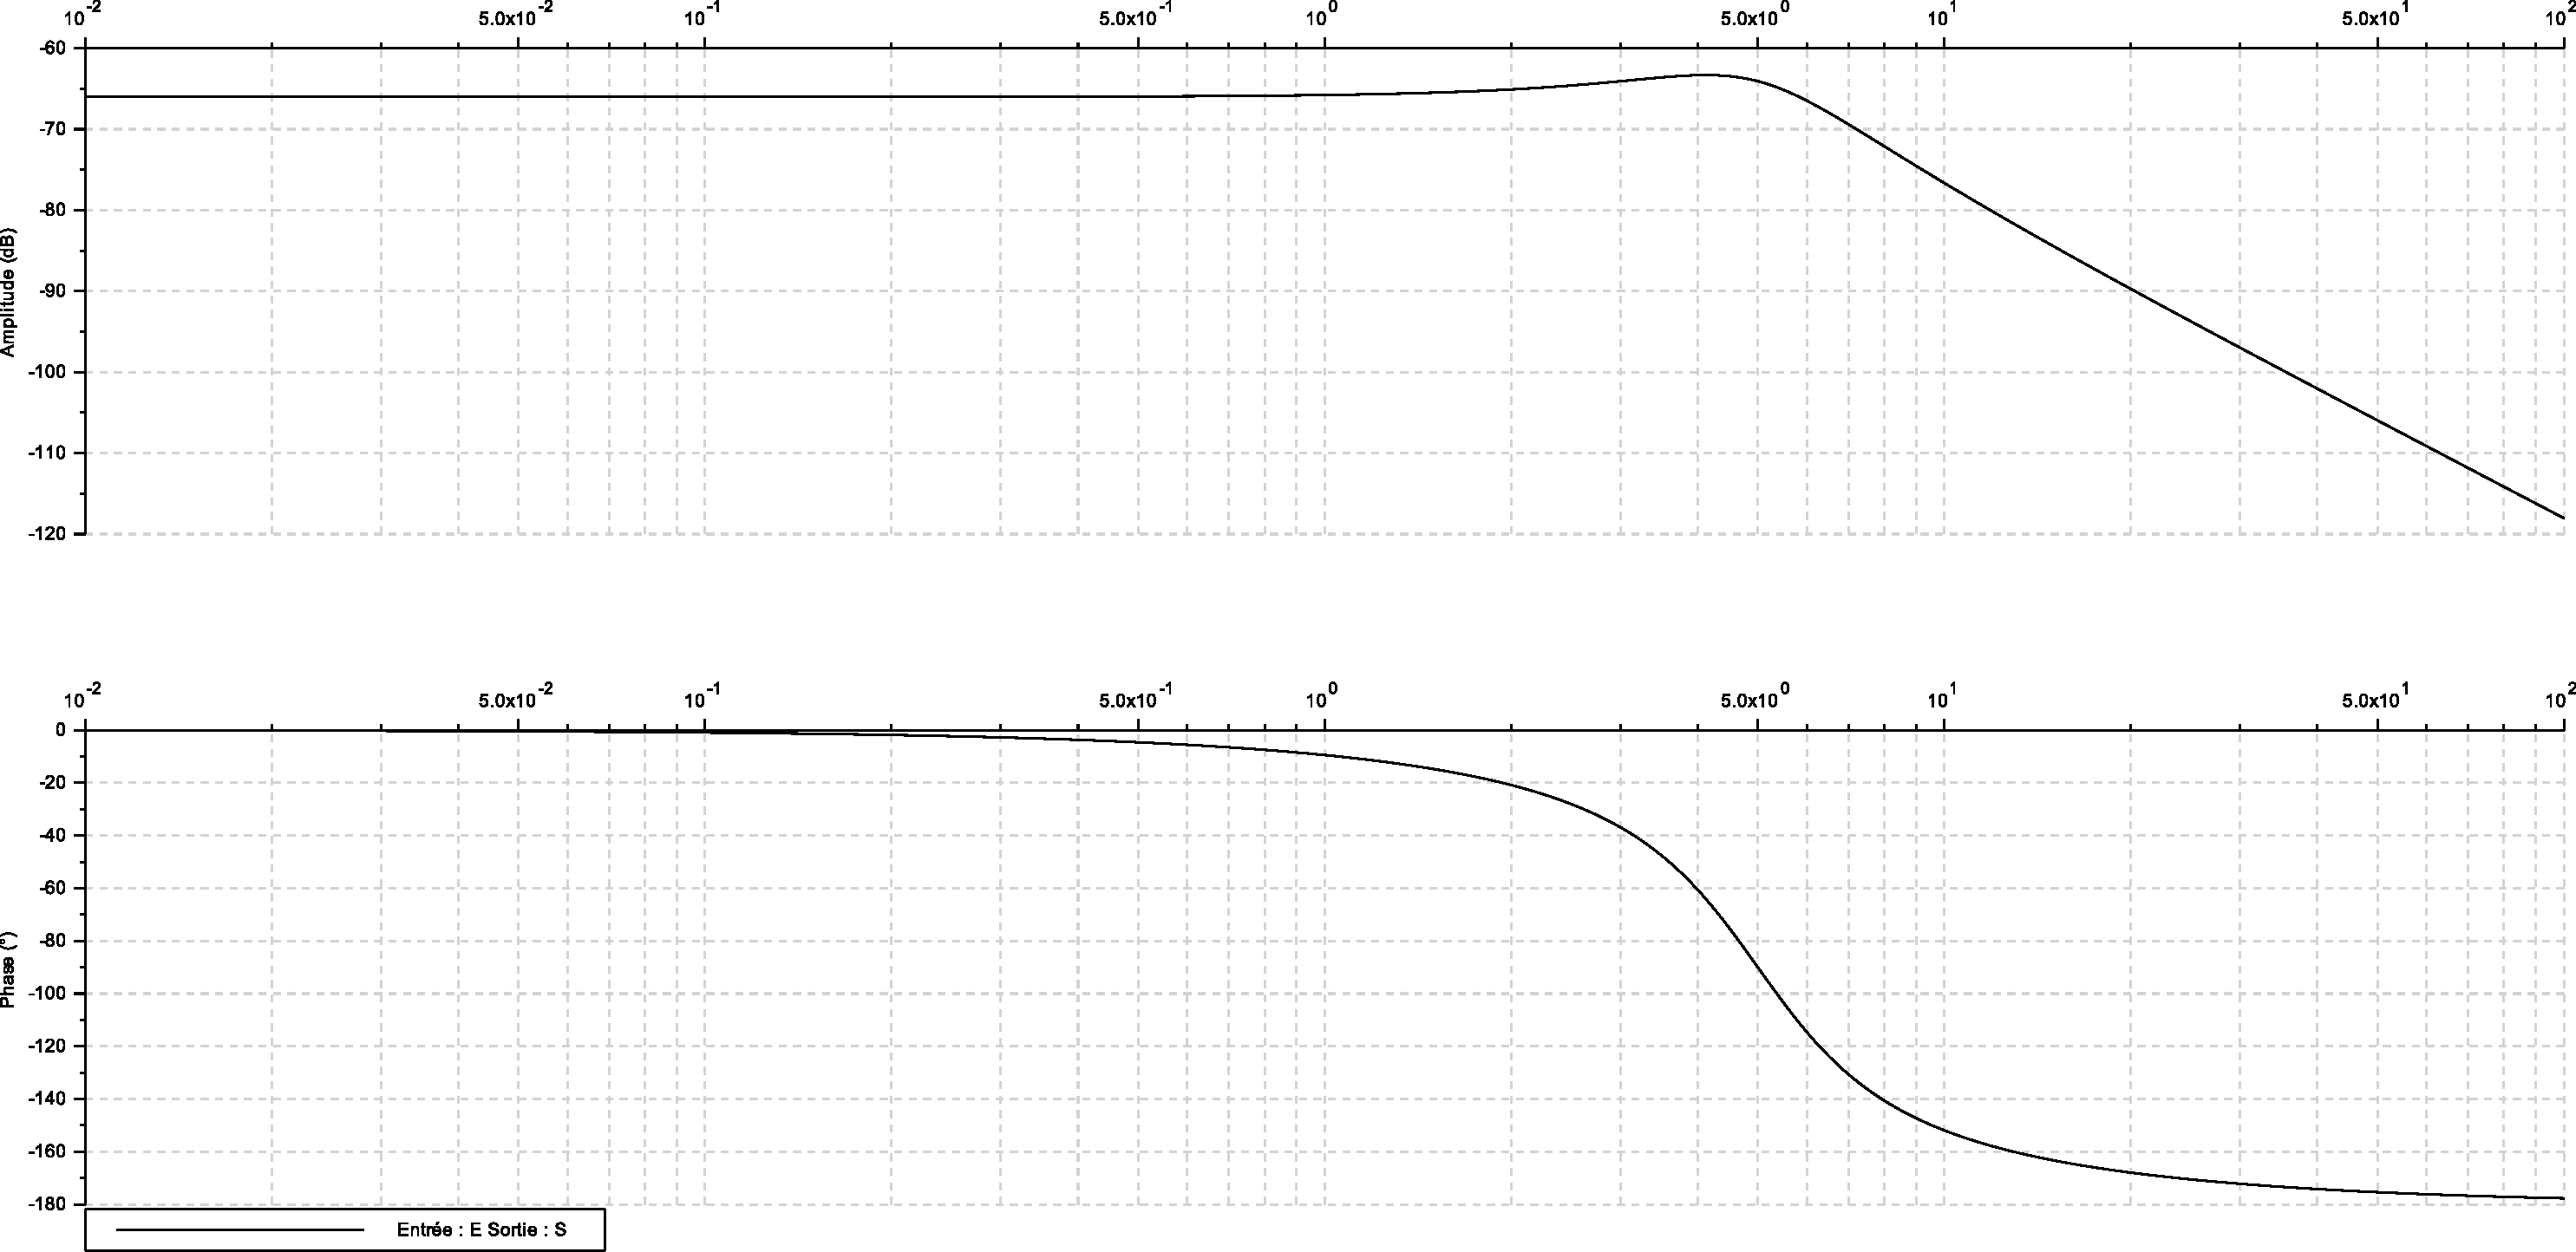
\includegraphics[width=0.8\linewidth]{img/03b}
 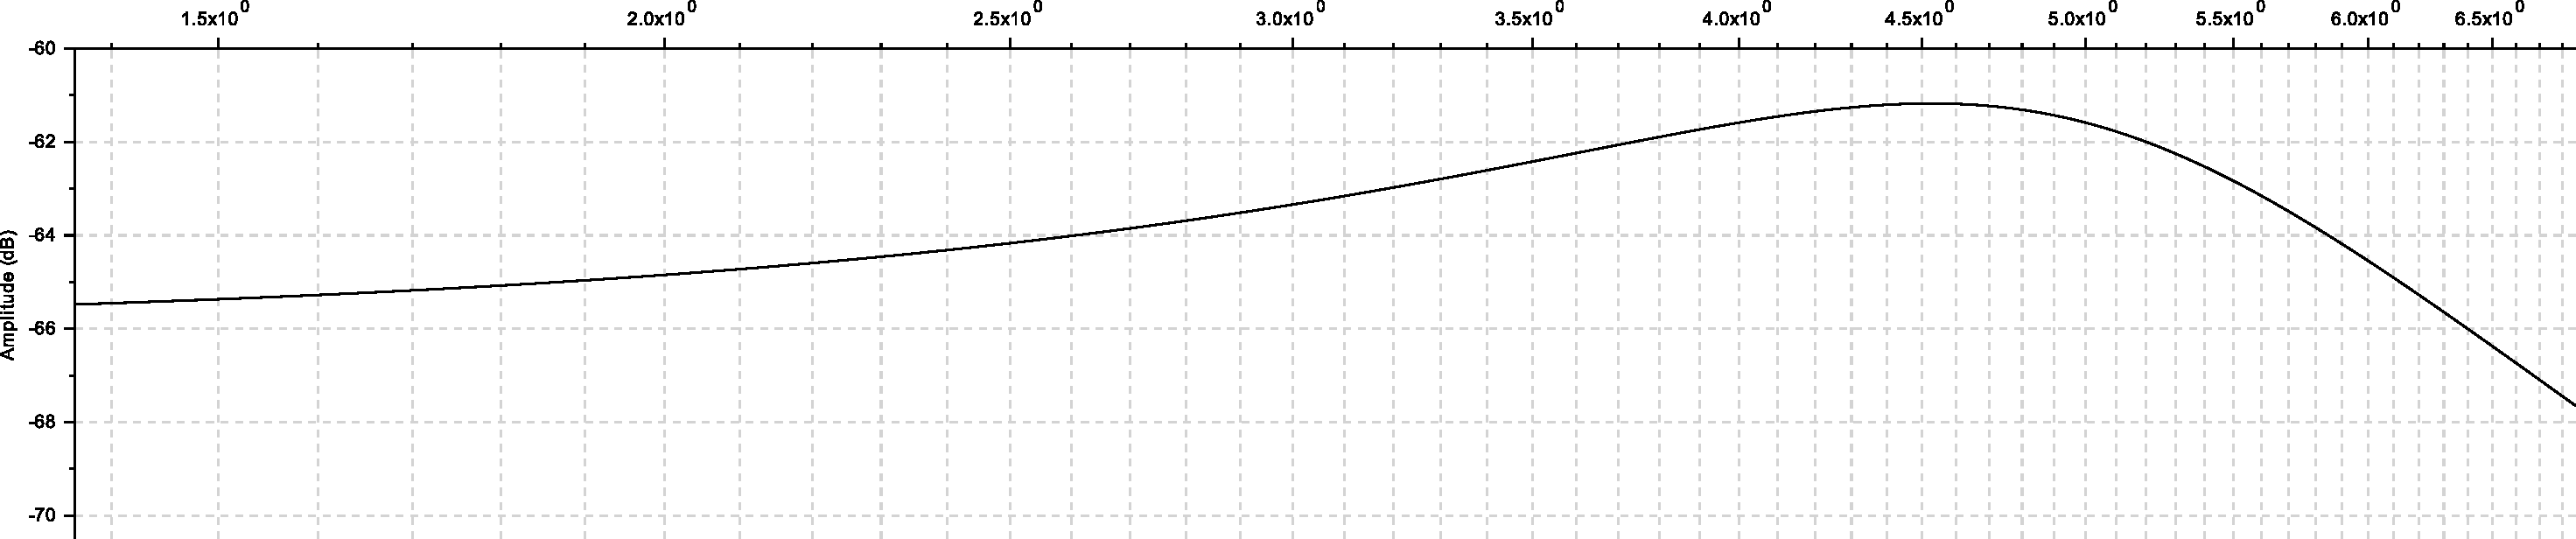
\includegraphics[width=0.8\linewidth]{img/03b_zoom}
\end{center}

\paragraph{Question 3:} Identifier la nouvelle fonction de transfert du système en question. Quel paramètre a été modifié par rapport à la précédente ?

\paragraph{Question 4:} L'exigence de la question 2 est-elle respectée ?

\paragraph{Question 5:} Une autre exigence du système consiste à exiger que la fourche soit revenue à +/- 5 mm de sa position de départ en moins de 0.5s. Cette exigence est-elle respectée ?

\newpage

\section{Asservissement des transferts thermiques dans un four industriel}

Une centrale nucléaire a pour fonction de produire de l'énergie électrique à partir d'énergie nucléaire.

\begin{center}
 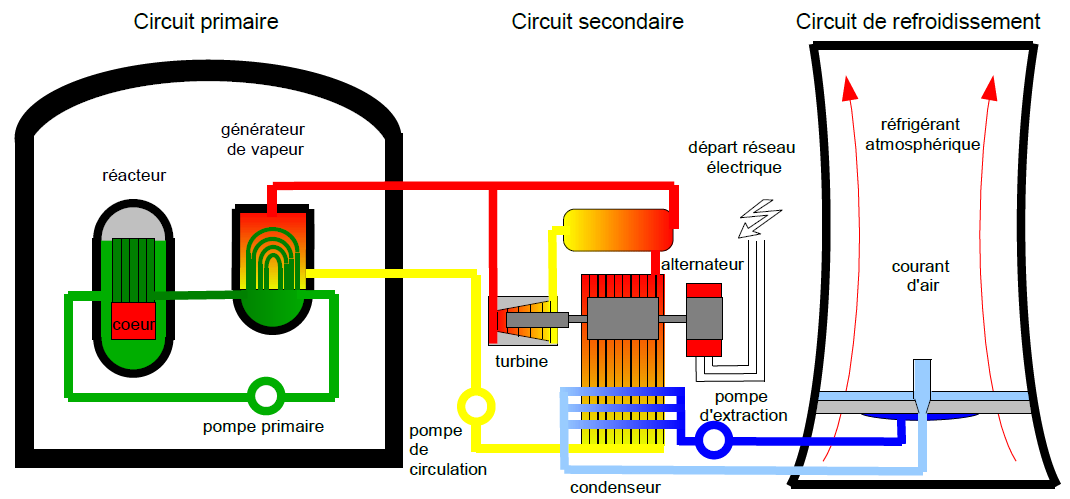
\includegraphics[width=0.8\linewidth]{img/fig3}
\end{center}

Le combustible nucléaire, contenu dans le c\oe ur du réacteur, chauffe un fluide caloriporteur dans le circuit primaire. La pompe primaire fait circuler ce fluide et l'emmène notamment dans les tuyaux du générateur de vapeur, au sein duquel il chauffe un autre fluide caloriporteur qui devient vapeur. Cette vapeur fait tourner une turbine qui génère de l'électricité via un alternateur. La vapeur va ensuite dans un condenseur pour être refroidie.

Les tubes du générateur de vapeur ont donc un rôle crucial dans le fonctionnement d'une centrale nucléaire.

\vfill

\begin{minipage}{0.4\linewidth}
 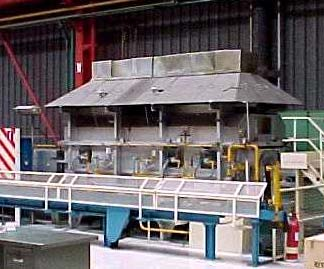
\includegraphics[width=0.8\linewidth]{img/fig4}
\end{minipage}
\hfill
\begin{minipage}{0.57\linewidth}
Pour obtenir des tubes de forme et de constitution moléculaire parfaites, les ingénieurs ont été amenés à imaginer une nouvelle technologie de four industriel permettant de chauffer les alliages de matériaux selon des processus bien définis. Ces fours peuvent fournir des températures de chauffe très précises grâce à un asservissement des transferts thermiques en leur sein.
\end{minipage}

\vfill

Faire un essai sur les conduites du four réel étant très coûteux, les ingénieurs ont décidé de réaliser leurs essais sur une maquette à échelle réduite, constituée d'un tube de conduite adiabatique, d'une résistance chauffante, d'un ventilateur (tournant à vitesse fixe, et permettant de faire circuler l'air), d'un volet réglable et d'un capteur de température. Ce système peut paraître simpliste au regard de la structure du four industriel, mais il permet de bien comprendre les phénomènes mis en jeu lors des transferts thermiques dans les conduites du four, et de poser les bonnes hypothèses pour les modéliser.

\begin{center}
 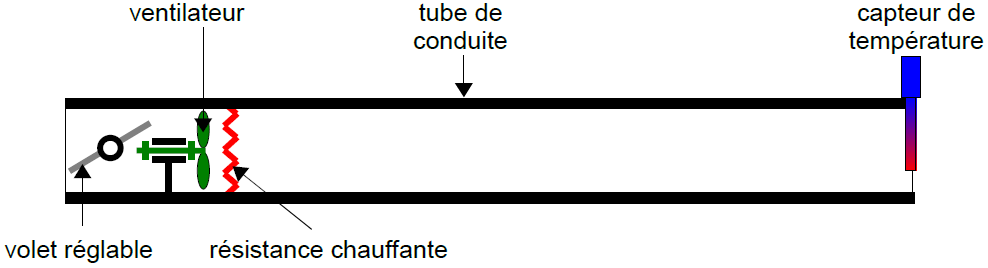
\includegraphics[width=0.9\linewidth]{img/fig5}
\end{center}

\subsection{Réponse expérimentale}

Les réponses expérimentales permettent de voir la propagation de la chaleur dans le tube de conduite, depuis l'instant $t=0$ (instant auquel la résistance chauffante et le ventilateur sont mis en marche). L'évolution de la température, au niveau du capteur de température, est représentée sur la figure suivante, la consigne pour cette réponse temporelle est un échelon de 40°.

\begin{center}
 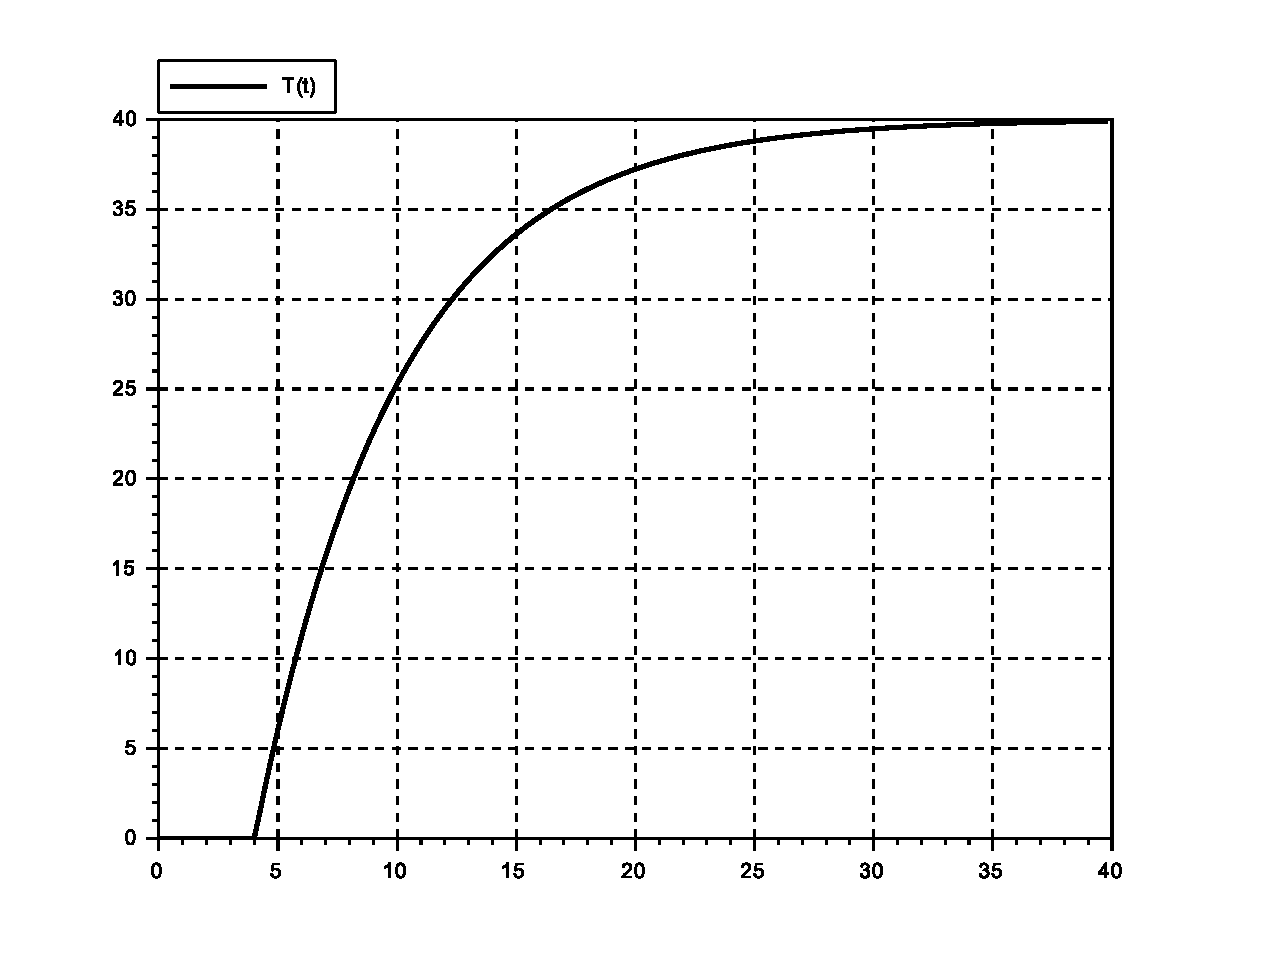
\includegraphics[width=0.9\linewidth]{img/04}
\end{center}

La figure présente l'évolution de la température $\theta_s(t)$, au niveau du capteur de température, après mise en marche de la résistance chauffante et du ventilateur à l'instant $t=0$. La température initiale dans le tube de conduite a été retranchée, ce qui explique la valeur $\theta_s(t)=0$ avant la mise en marche de la résistance de chauffe.

\paragraph{Question 1:} Comment expliquer la réponse jusqu'à t=4s?

\paragraph{Question 2:} Déterminer la fonction de transfert de ce système.

\paragraph{Question 3:} Ce genre de système peut parfois être considéré comme difficile à asservir, expliquer pourquoi.

\paragraph{Question 4:} Donner le temps de réponse $t_{5\%}$. Le cahier des charges exige $t_{5\%}<25s$, cette valeur est-elle respectée ?

\newpage

\subsection{Tracé de diagrammes}

\paragraph{Question 1:} Tracer les diagrammes de Bode de la fonction de transfert $H_1(p)$.

\begin{center}
$H_1(p)=\frac{10}{1+2.\frac{4}{100}.p+\frac{p^2}{100^2}}$
\end{center}

\begin{center}
 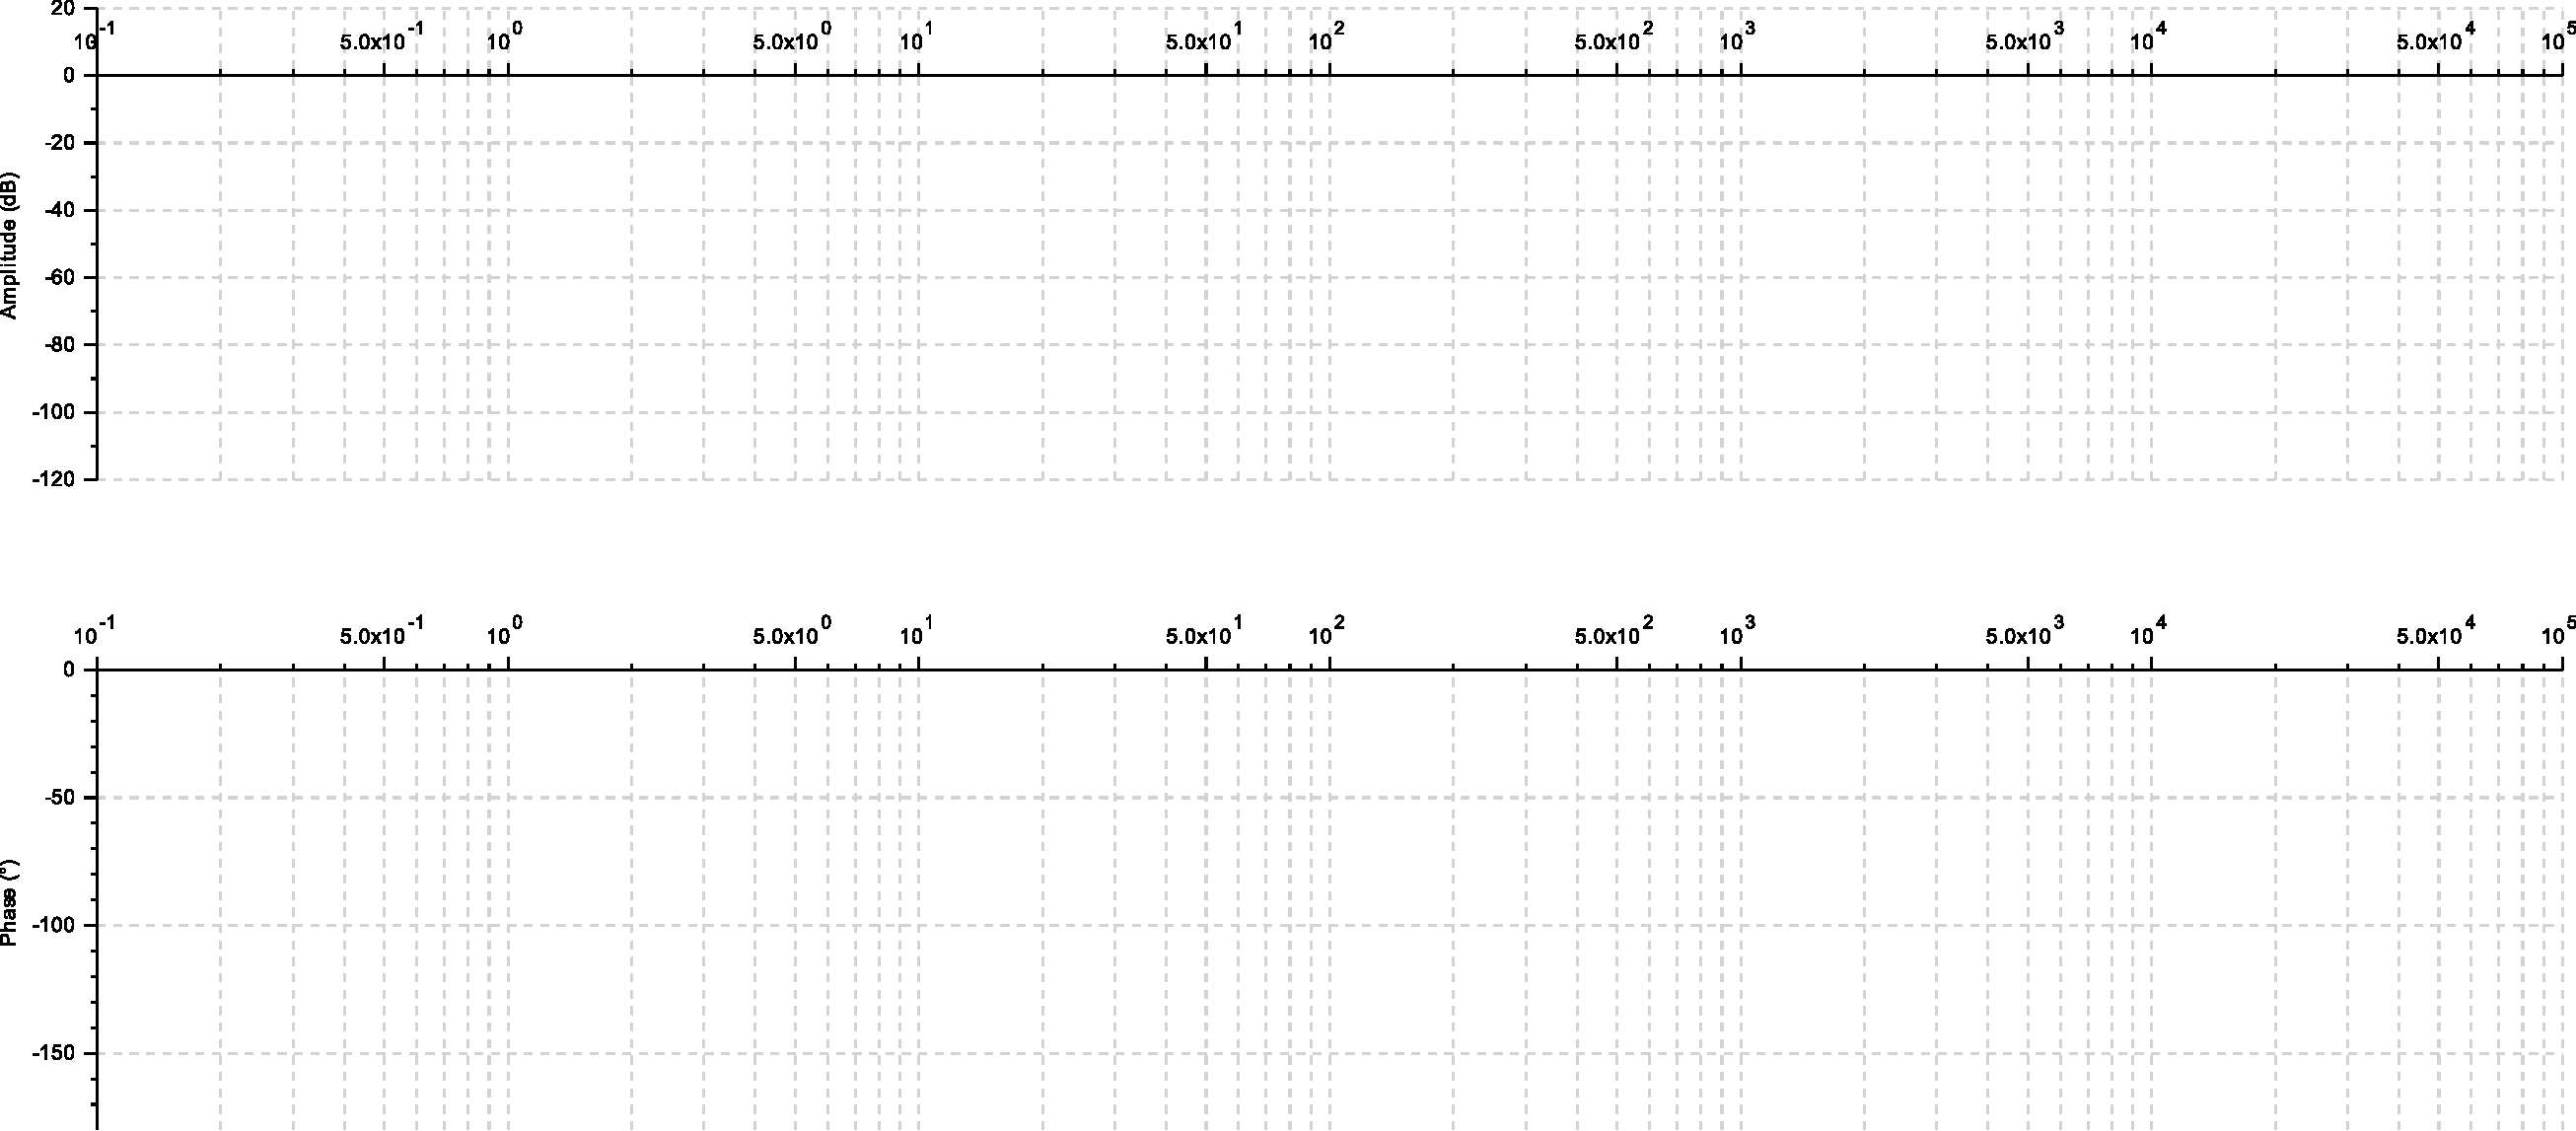
\includegraphics[width=0.9\linewidth]{img/BodeH1}
\end{center}

\paragraph{Question 2:} Tracer les diagrammes de Bode de la fonction de transfert $H_2(p)$.

\begin{center}
$H_2(p)=\frac{40}{1+0,01.p+\frac{p^2}{90^2}}$
\end{center}

\begin{center}
 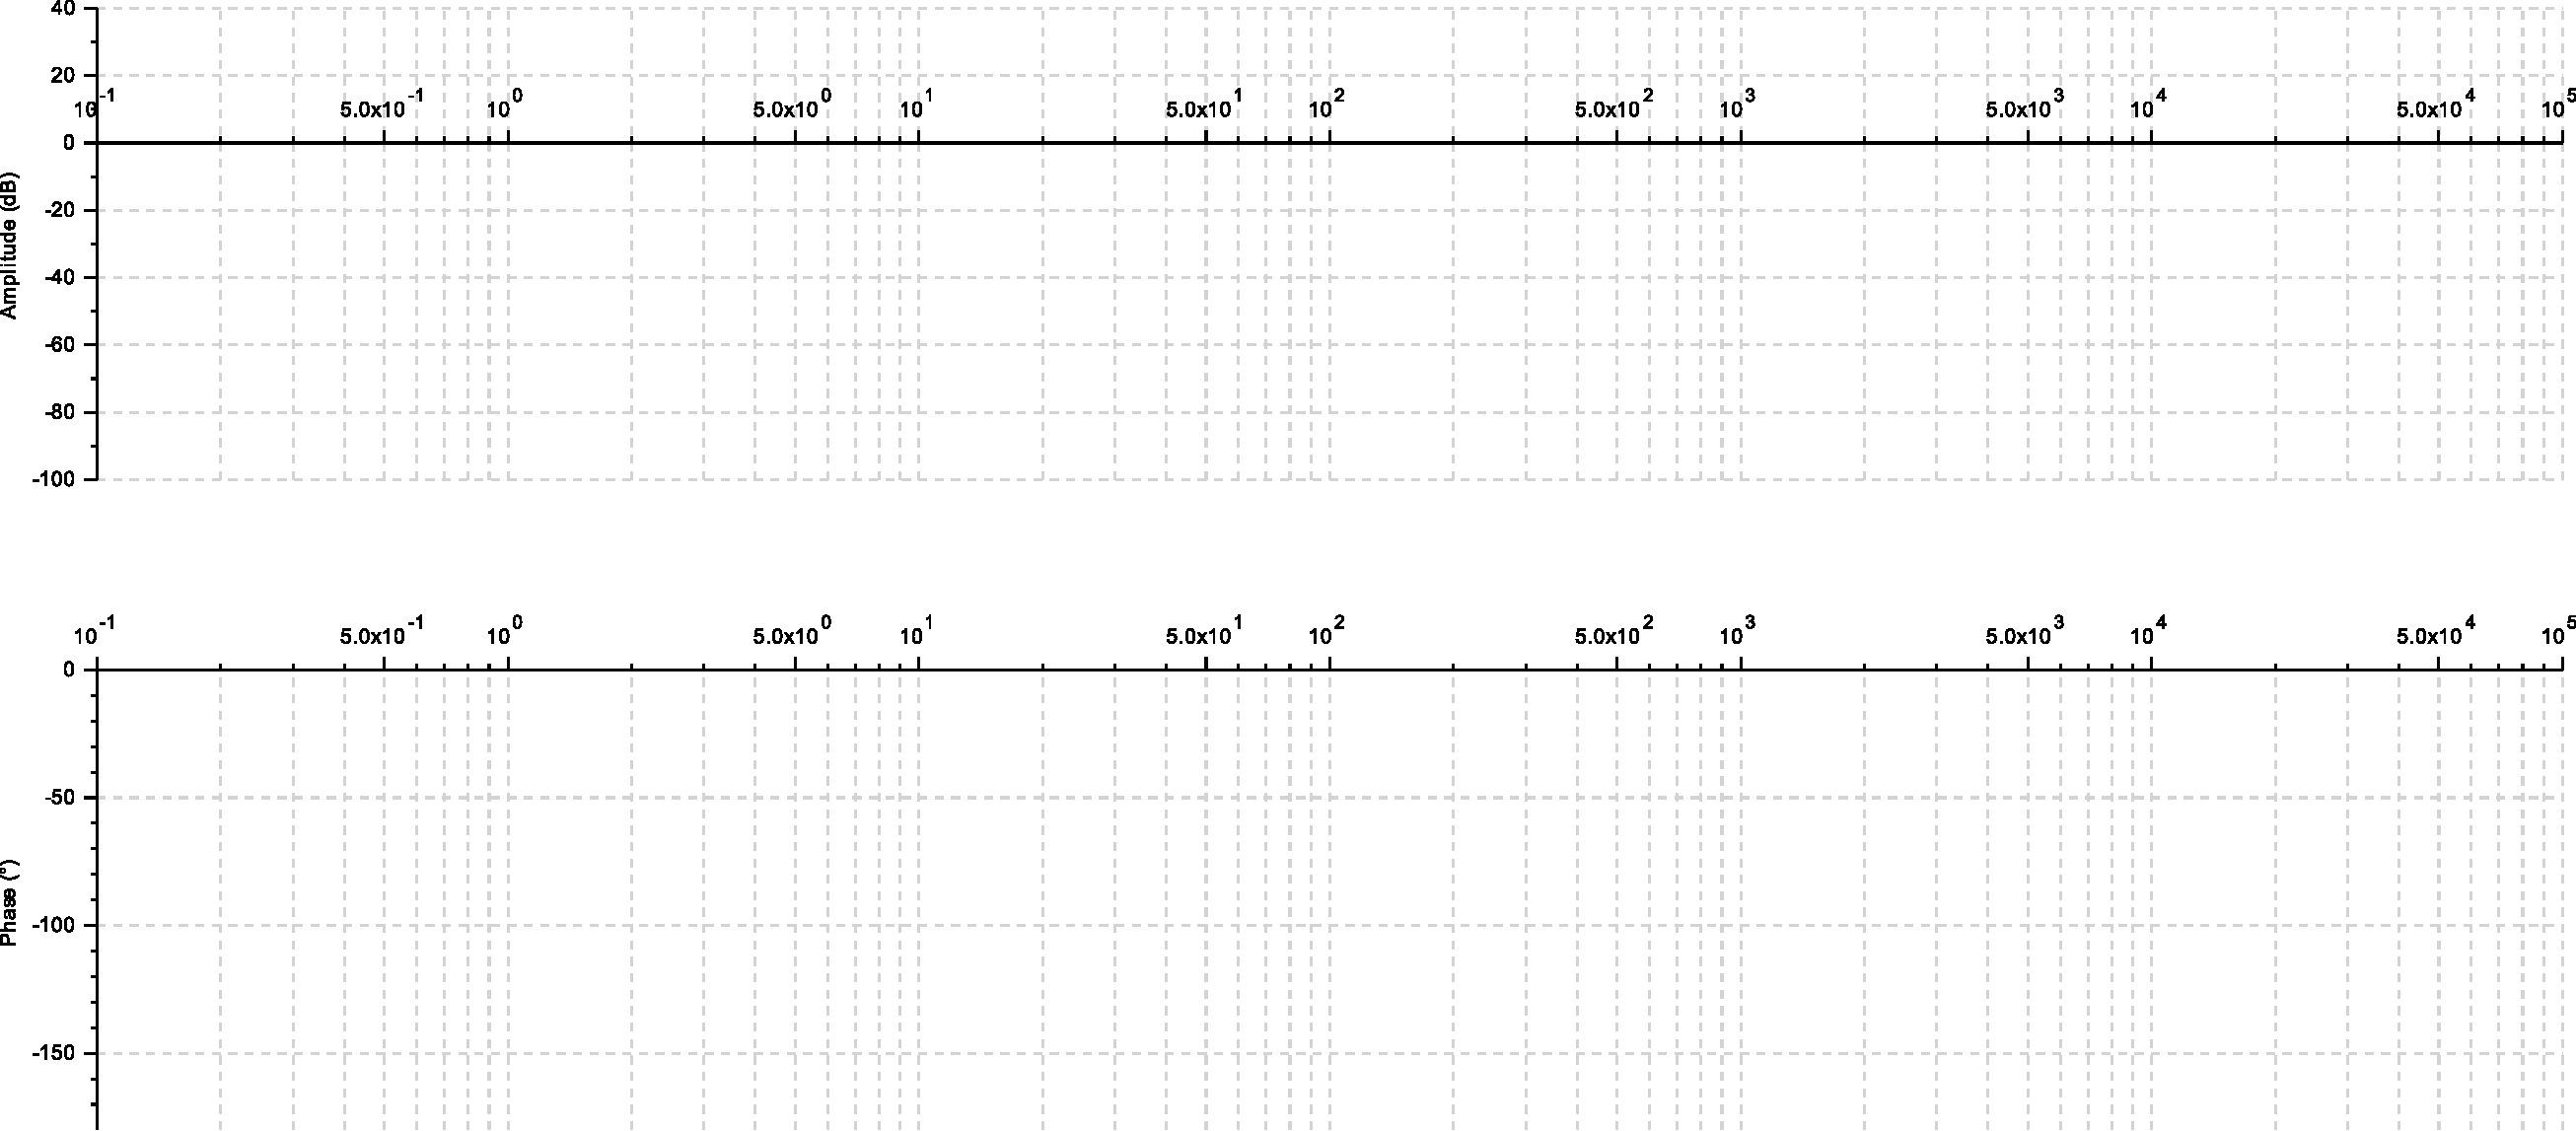
\includegraphics[width=0.9\linewidth]{img/BodeH2}
\end{center}

\ifdef{\public}{\end{document}}{}

\newpage

\pagestyle{correction}

\section{Correction}

\subsection{Circuit RC}

\paragraph{Question 1:}

\begin{center}
 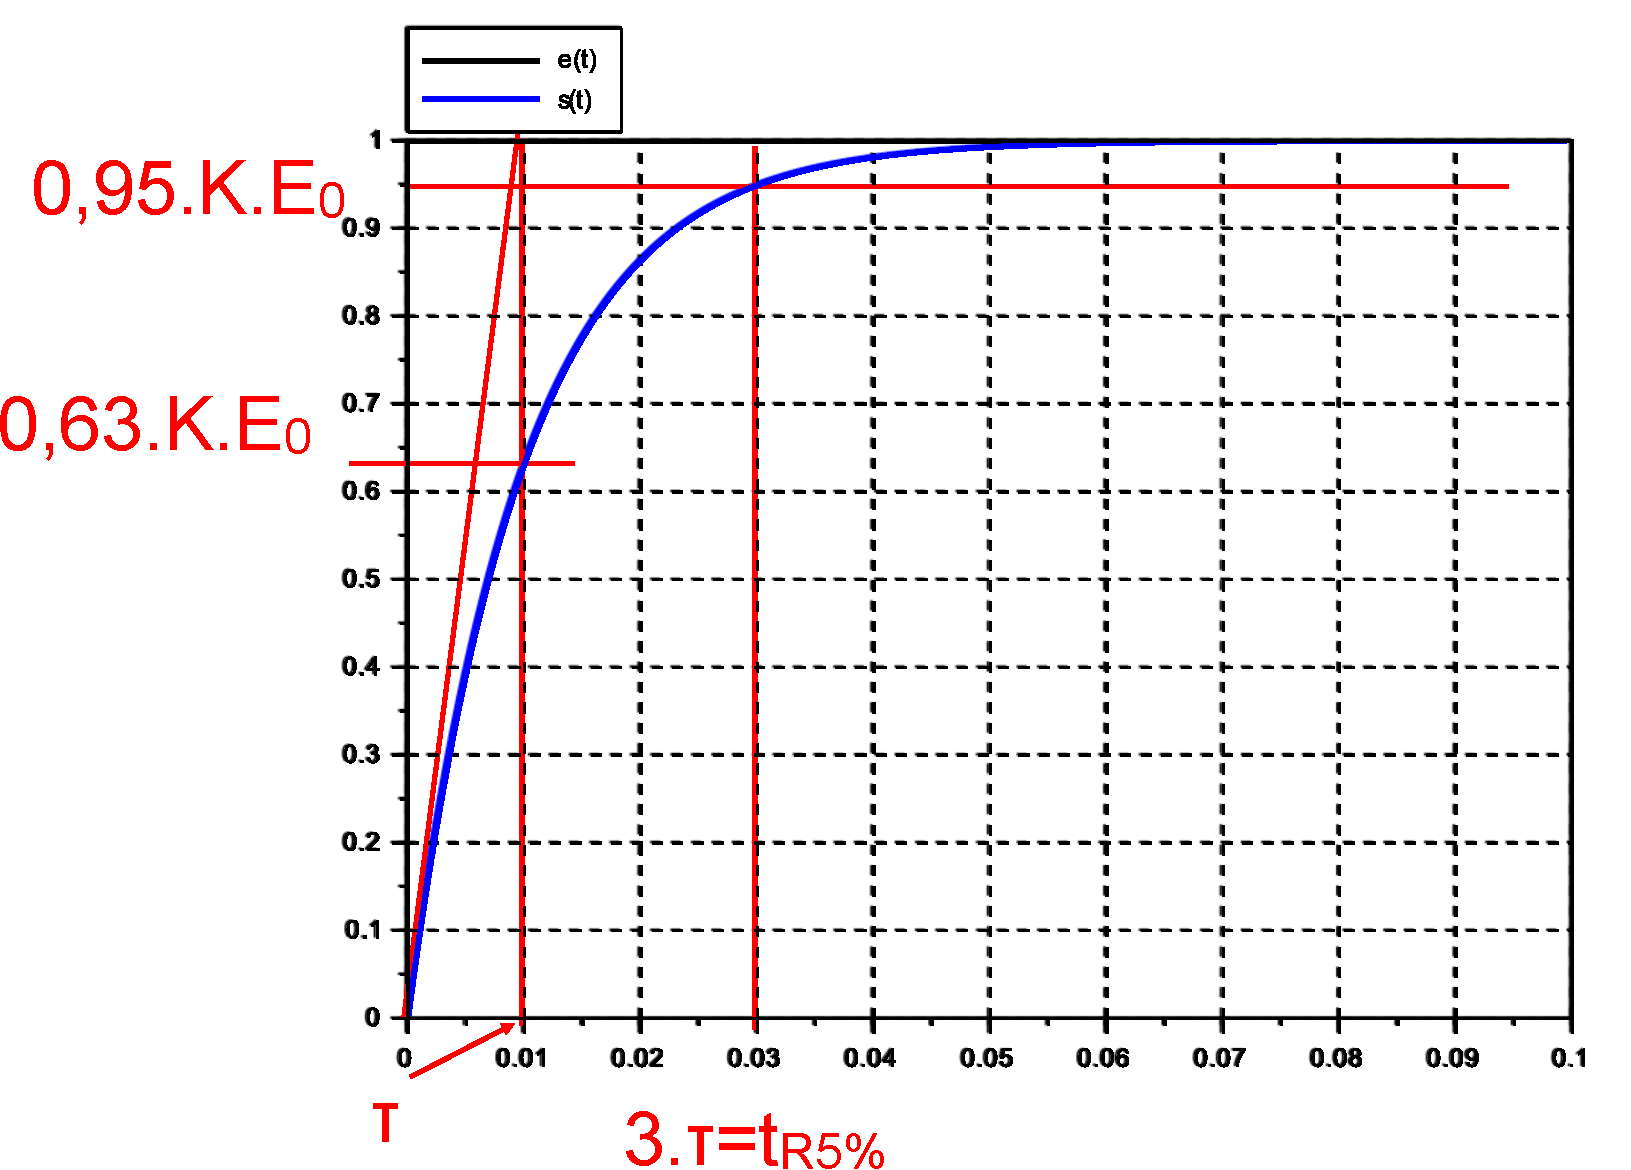
\includegraphics[width=0.7\linewidth]{img/exo_1_cor}
\end{center}

$H(p)=\dfrac{1}{1+0,01.p}$

\paragraph{Question 2:}

$t_{R,5\%}=0,03s<0,06s$, le système respect ainsi le cahier des charges.

\subsection{Amortisseur mécanique}

\paragraph{Question 1:}

\begin{center}
 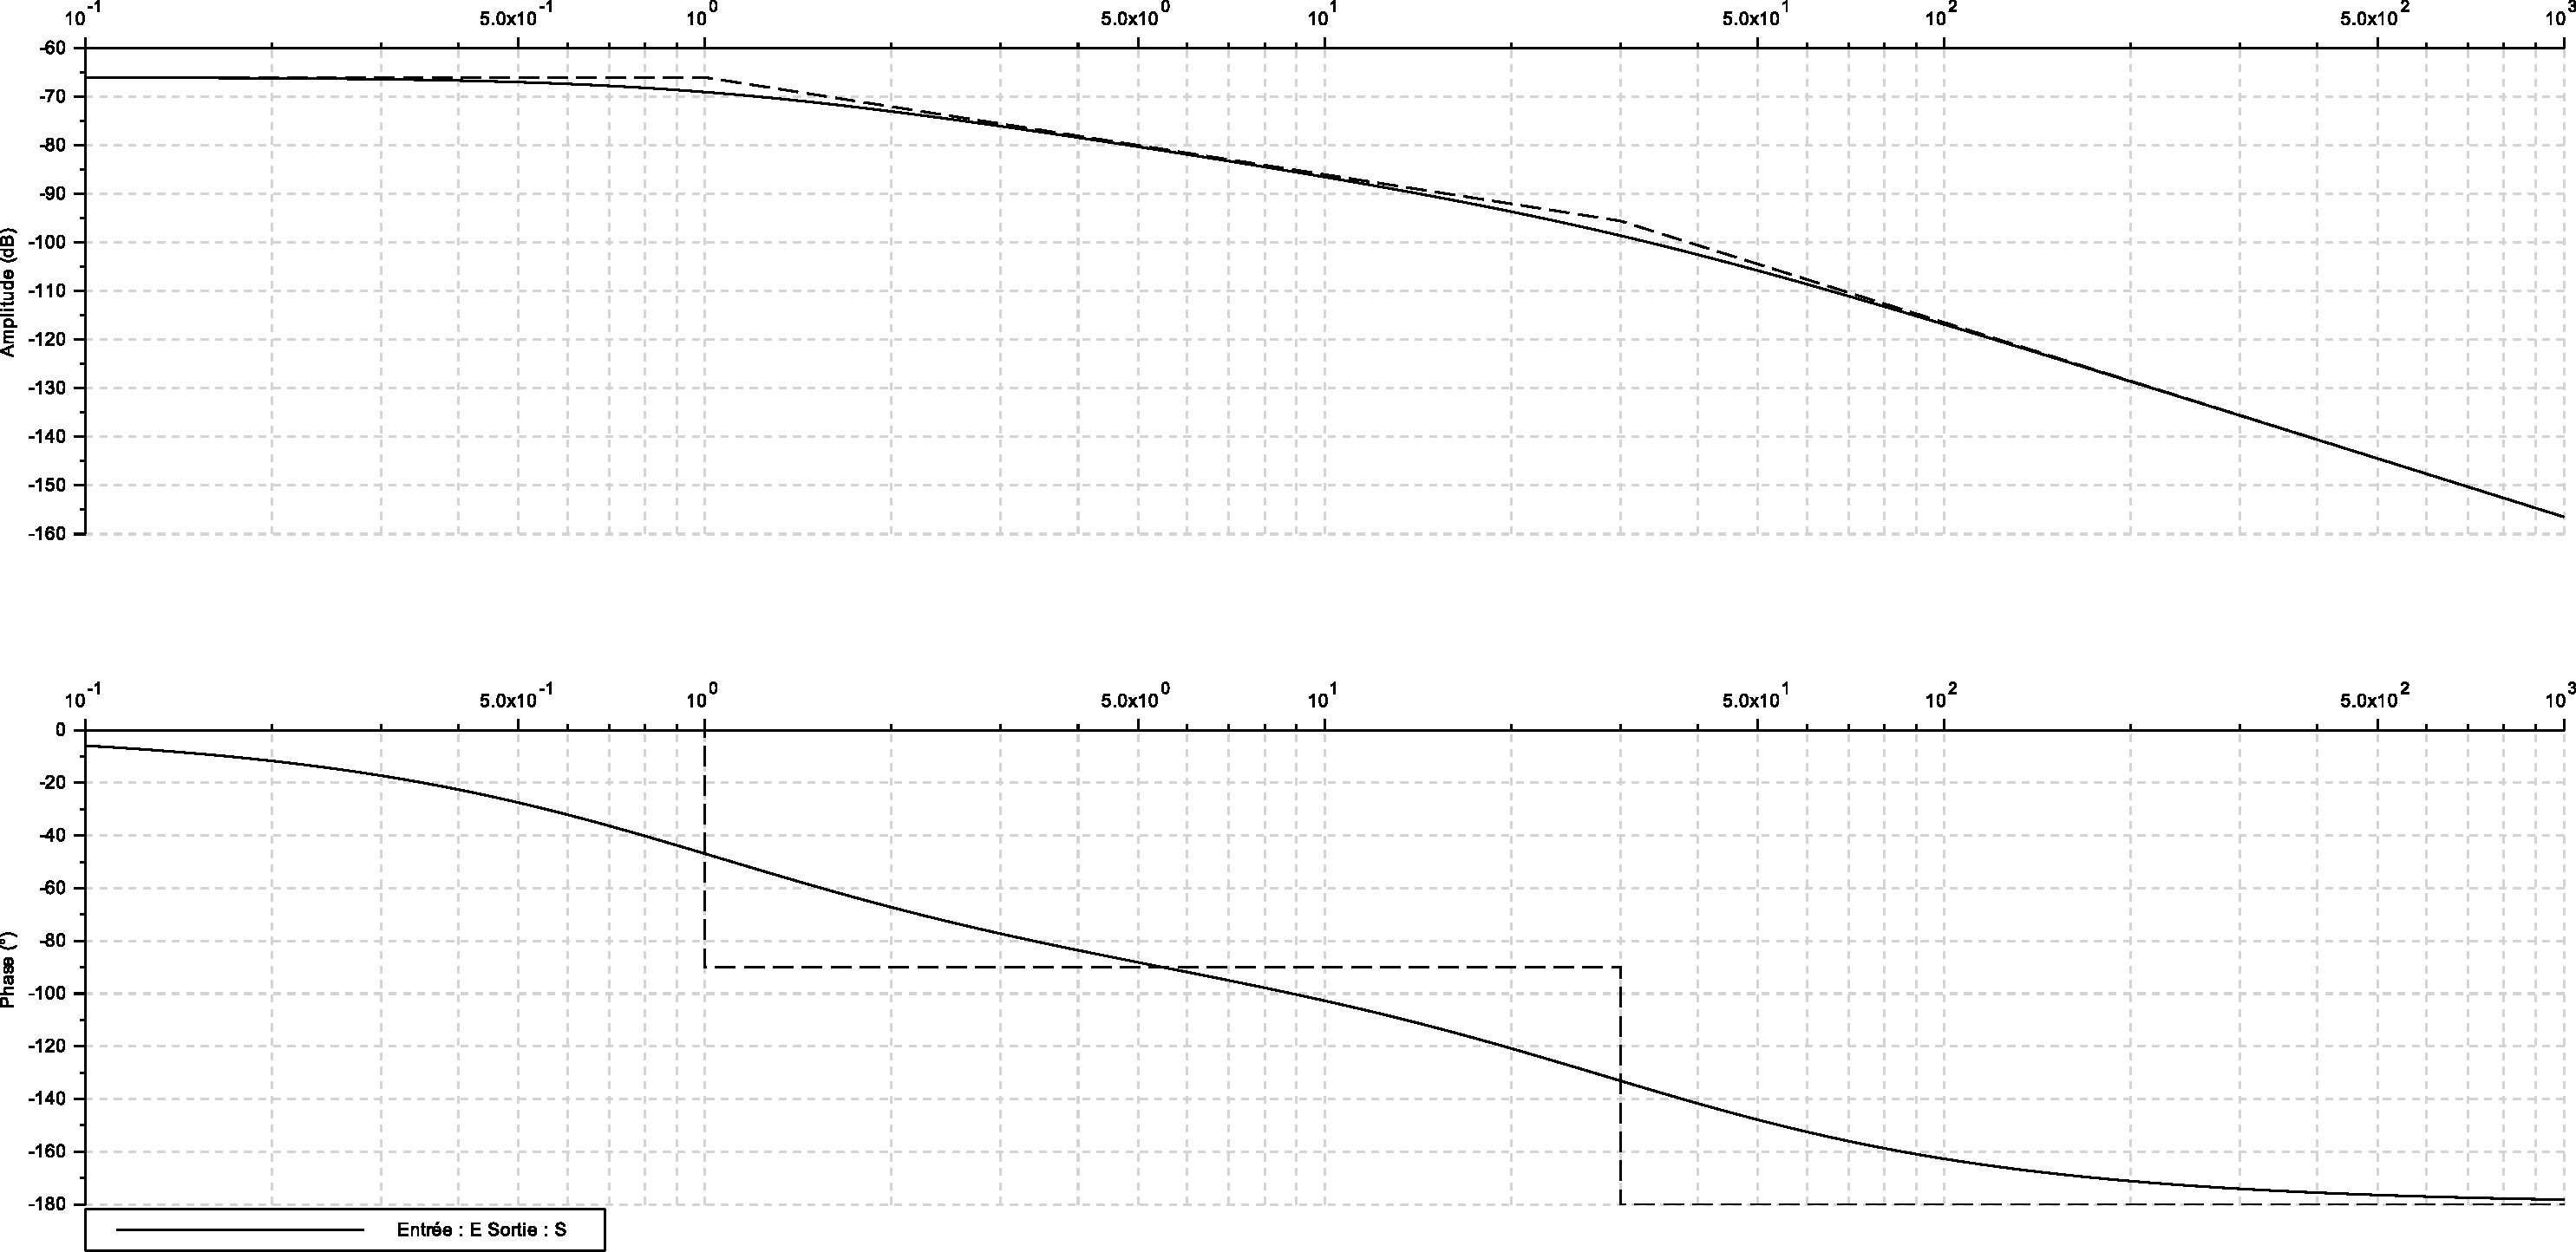
\includegraphics[width=0.8\linewidth]{img/exo_2_cor}
\end{center}

\begin{minipage}{0.5\linewidth}
\begin{itemize}
 \item $\omega_1=1rad.s^{-1}$ et $\omega_2=30rad.s^{-1}$
 \item $20.log(K)=-66dB$, donc $K=5.10^{-4}$.
 \item Donc, $\omega_0=5,5rad.s^{-1}$ et $\xi=2,83$.
\end{itemize}
\end{minipage}\hfill
\begin{minipage}{0.4\linewidth}
$H(p)=\dfrac{5.10^{-4}}{(1+p).(1+\dfrac{p}{30})}$
\end{minipage}

\paragraph{Question 2:}

Pour un effort de $10N$, le déplacement est de $4,5mm$, ce qui signifie que pour 100N, il sera de $4,5cm>1,5cm$, le système ne respecte pas le cahier des charges.

\paragraph{Question 3:}

\begin{center}
 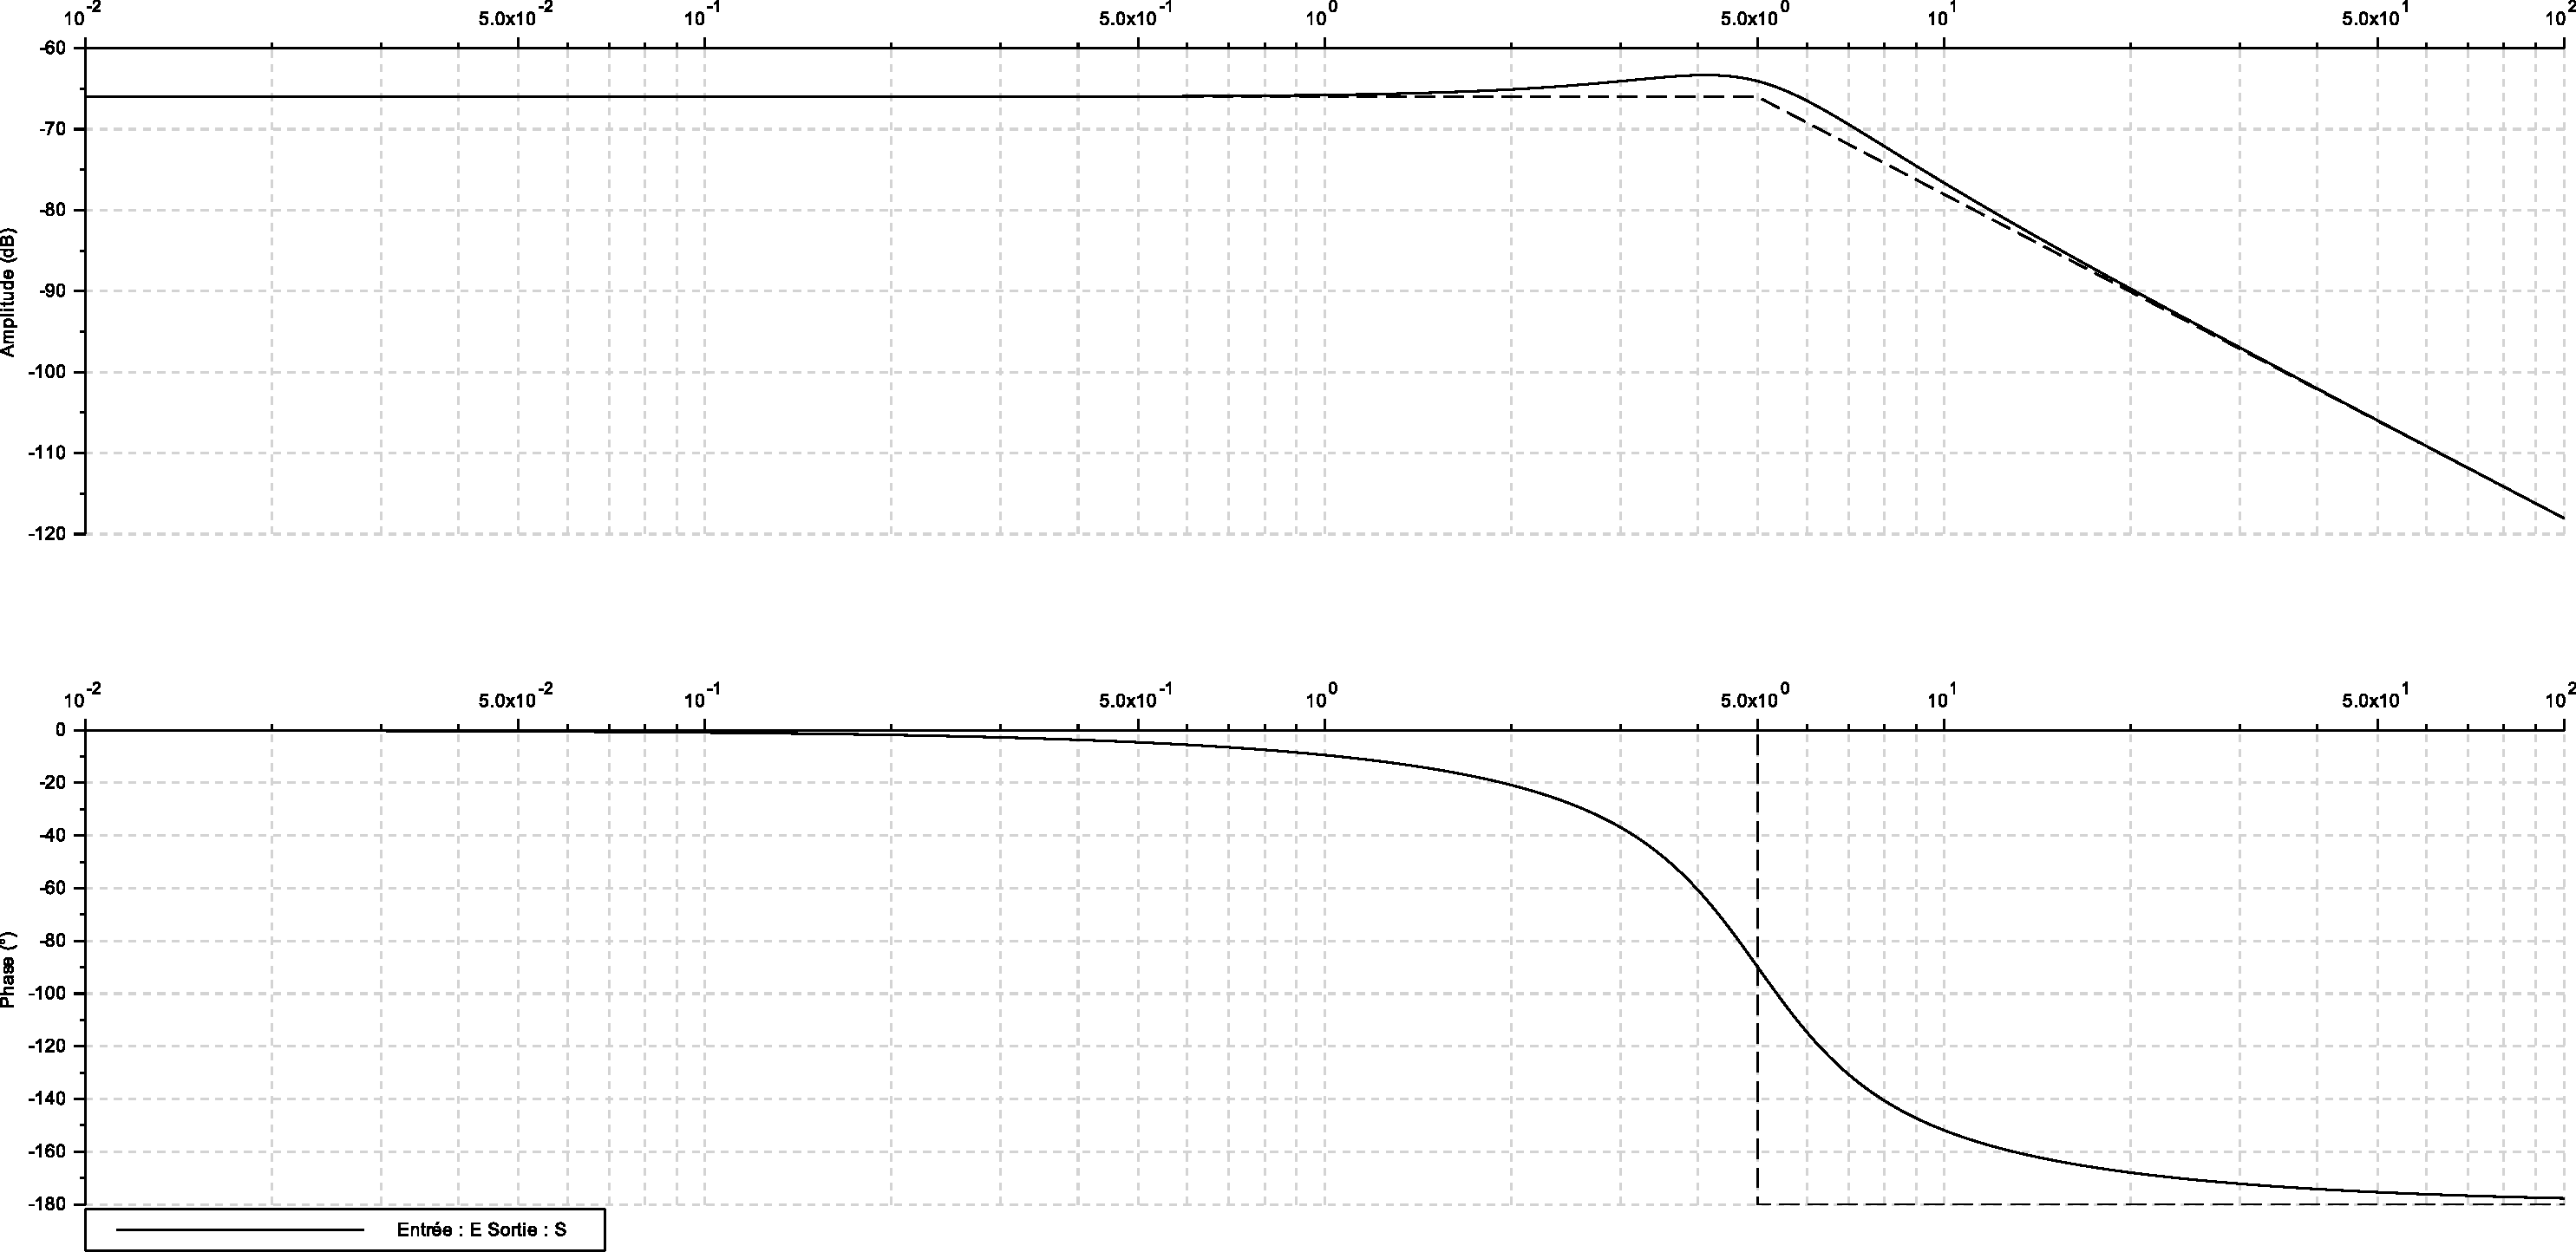
\includegraphics[width=0.8\linewidth]{img/exo_2_2_cor}\\
 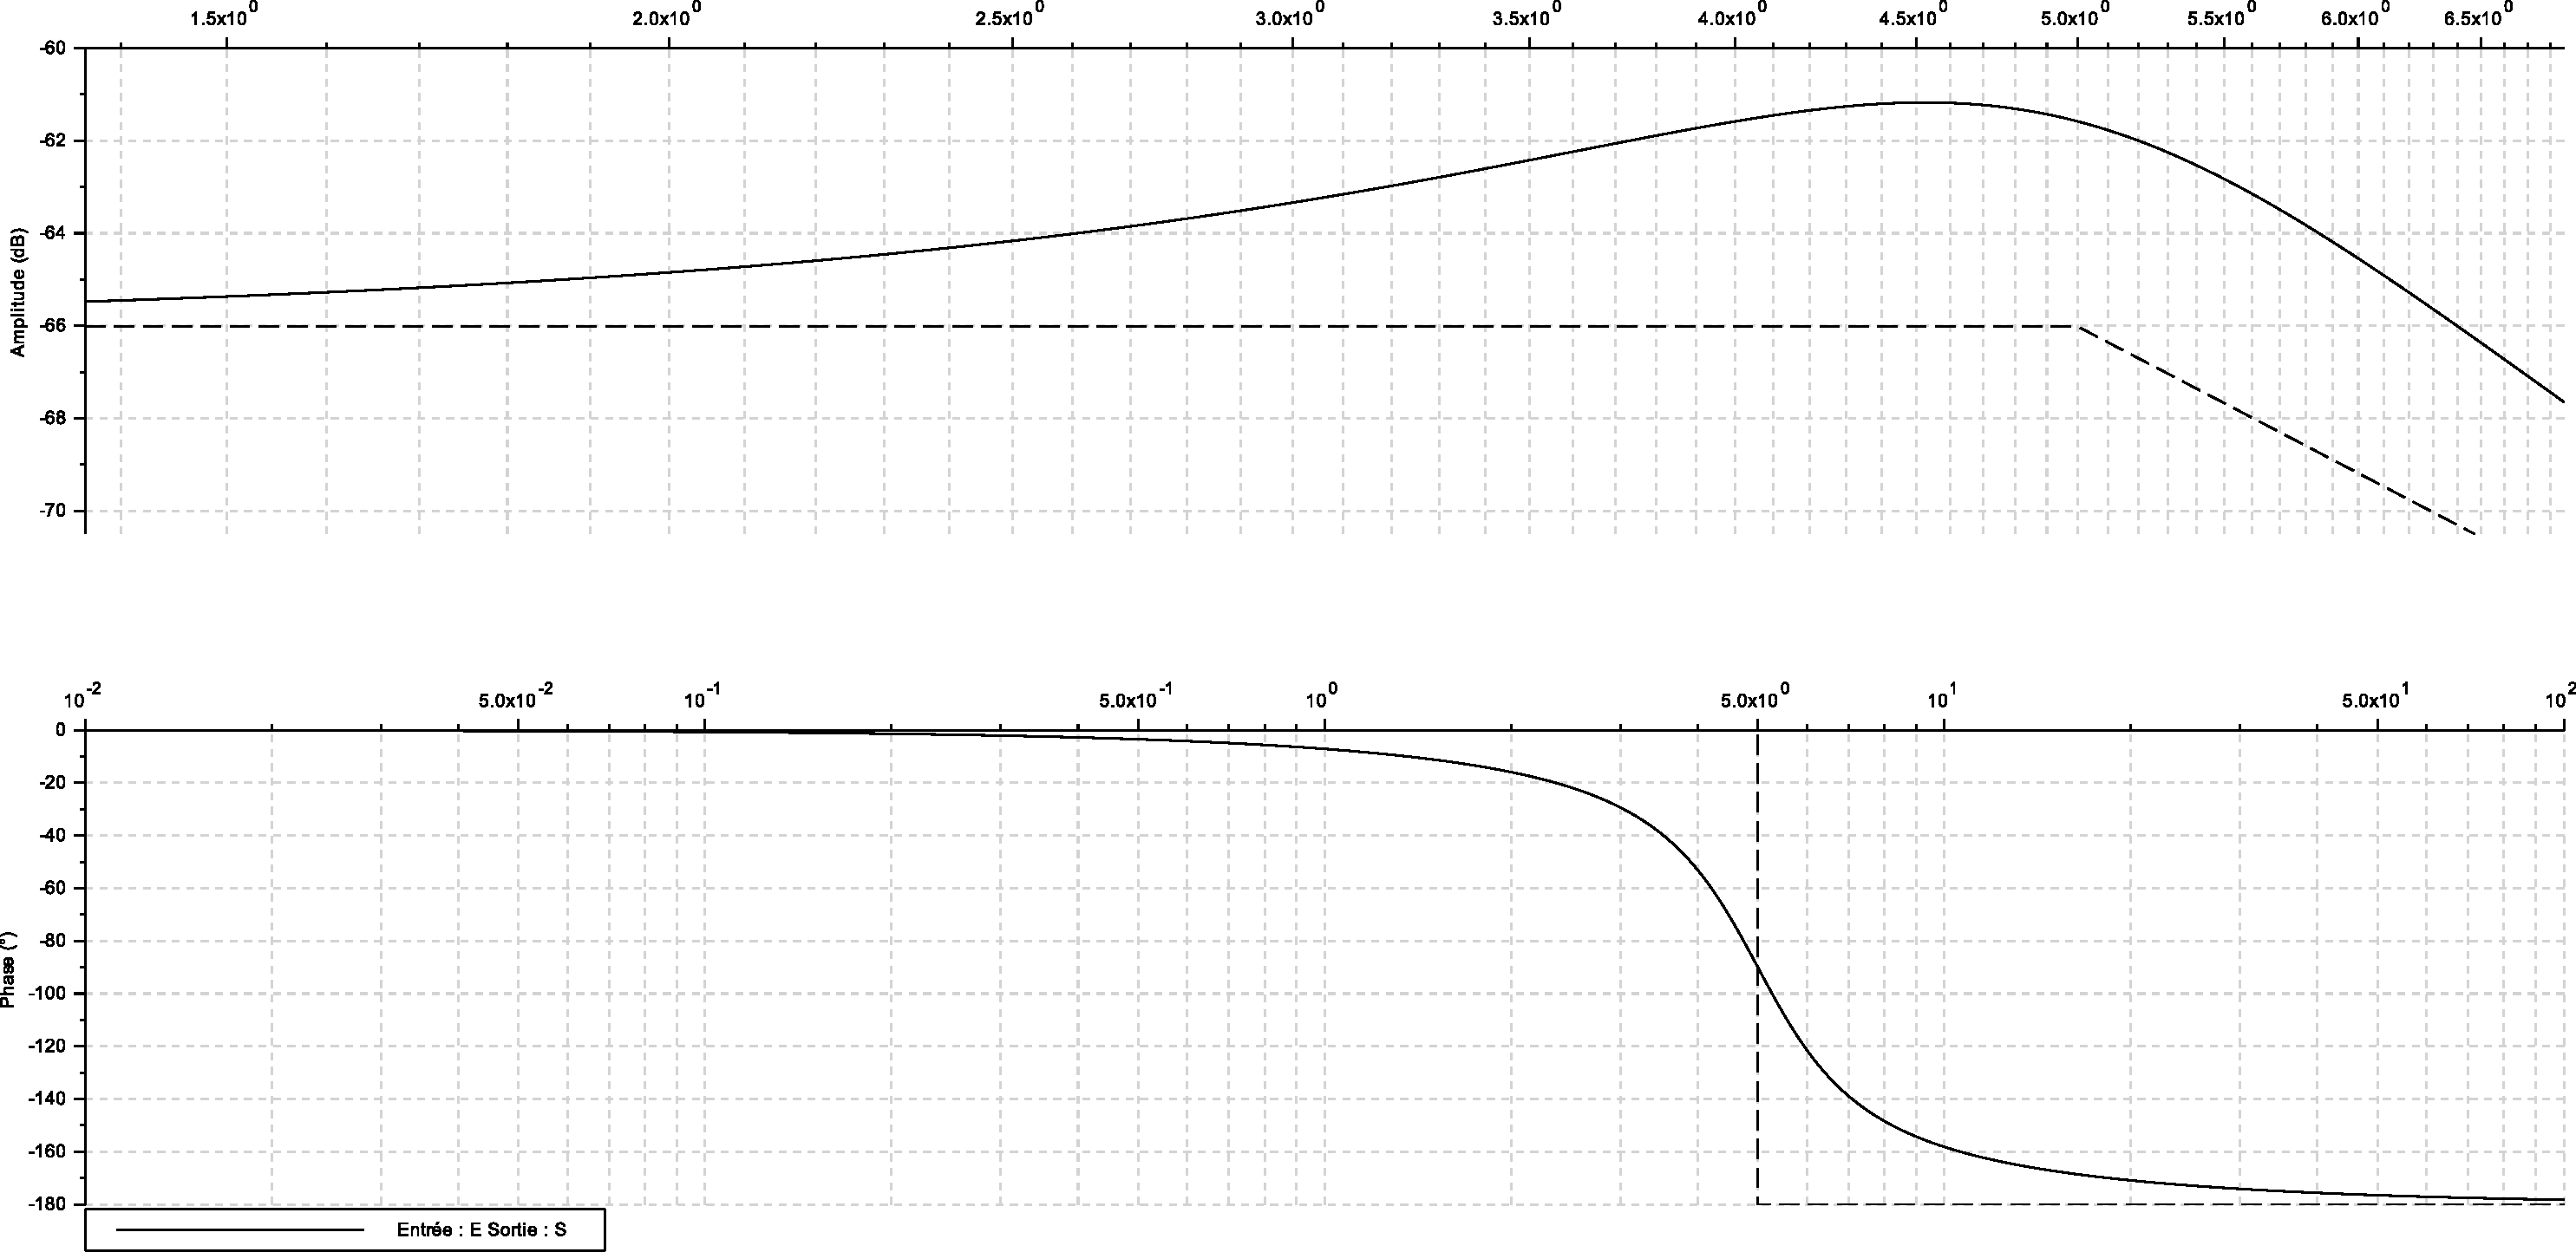
\includegraphics[width=0.8\linewidth]{img/exo_2_2_cor_zoom}
\end{center}

\begin{minipage}{0.45\linewidth}
$Q_{dB}=5$ \\
$Q=10^{\frac{5}{20}}=1,78$\\
$Q=1,78=\frac{1}{2.z.\sqrt{1-z^2}}$ \\
$z.\sqrt{1-z^2}=\frac{1}{2*1,78}$ \\
$z^2-z^4=0,08$ \\
Soit $X=z^2$ \\
$X^2-X+0,08=0$
\end{minipage}\hfill
\begin{minipage}{0.45\linewidth}
$\Delta=1-4*0,08=0,68$ \\
$x_1=\frac{1+sqrt{0,68}}{2}=0,91$ \\
$x_2=\frac{1-sqrt{0,68}}{2}=0,09$ \\
$z_1=0,96$ \\
$z_2=0,3$
\end{minipage}

La valeur ne pouvant pas se trouver entre $0,69$ et $1$ car il y a une résonance. Ainsi, $z=0,3$.

\begin{minipage}{0.45\linewidth}
$\omega_R=\omega_0.\sqrt{1-2.z^2}$ \\
$1-2.z^2=\left(\frac{\omega_R}{\omega_0}\right)^2$
\end{minipage}\hfill
\begin{minipage}{0.45\linewidth}
$z=\sqrt{\dfrac{1-\left(\frac{\omega_R}{\omega_0}\right)^2}{2}}$\\
$z=\sqrt{\dfrac{1-\left(\frac{4,5}{5}\right)^2}{2}}=0,3$
\end{minipage}

On retrouve la valeur $z=0,3$.

\paragraph{Question 4:}

Dans ce cas, le résultat valide le cahier des charges.

\paragraph{Question 5:}

L'exigence est respectée.

\subsection{Four industriel}

\paragraph{Question 1:}

Le décalage de la réponse est un retard du à la distance entre la résistance et le capteur.

\paragraph{Question 2:}

$H(p)=\frac{1}{1+6*p}.e^{-4.p}$

\paragraph{Question 3:}

Ce genre de système peut être considéré comme difficile à asservir car à cause du retard, les effets des corrections ne sont pas visibles instantanément.

\paragraph{Question 4:}

Le temps de réponse est de 24s, cela respecte le cahier des charges.

\subsection{Tracé de diagrammes}

\paragraph{Question 1:} Tracer les diagrammes de Bode de la fonction de transfert $H_1(p)$.

\begin{center}
$H_1(p)=\frac{10}{1+2.\frac{4}{100}.p+\frac{p^2}{100^2}}$
\end{center}

\begin{center}
 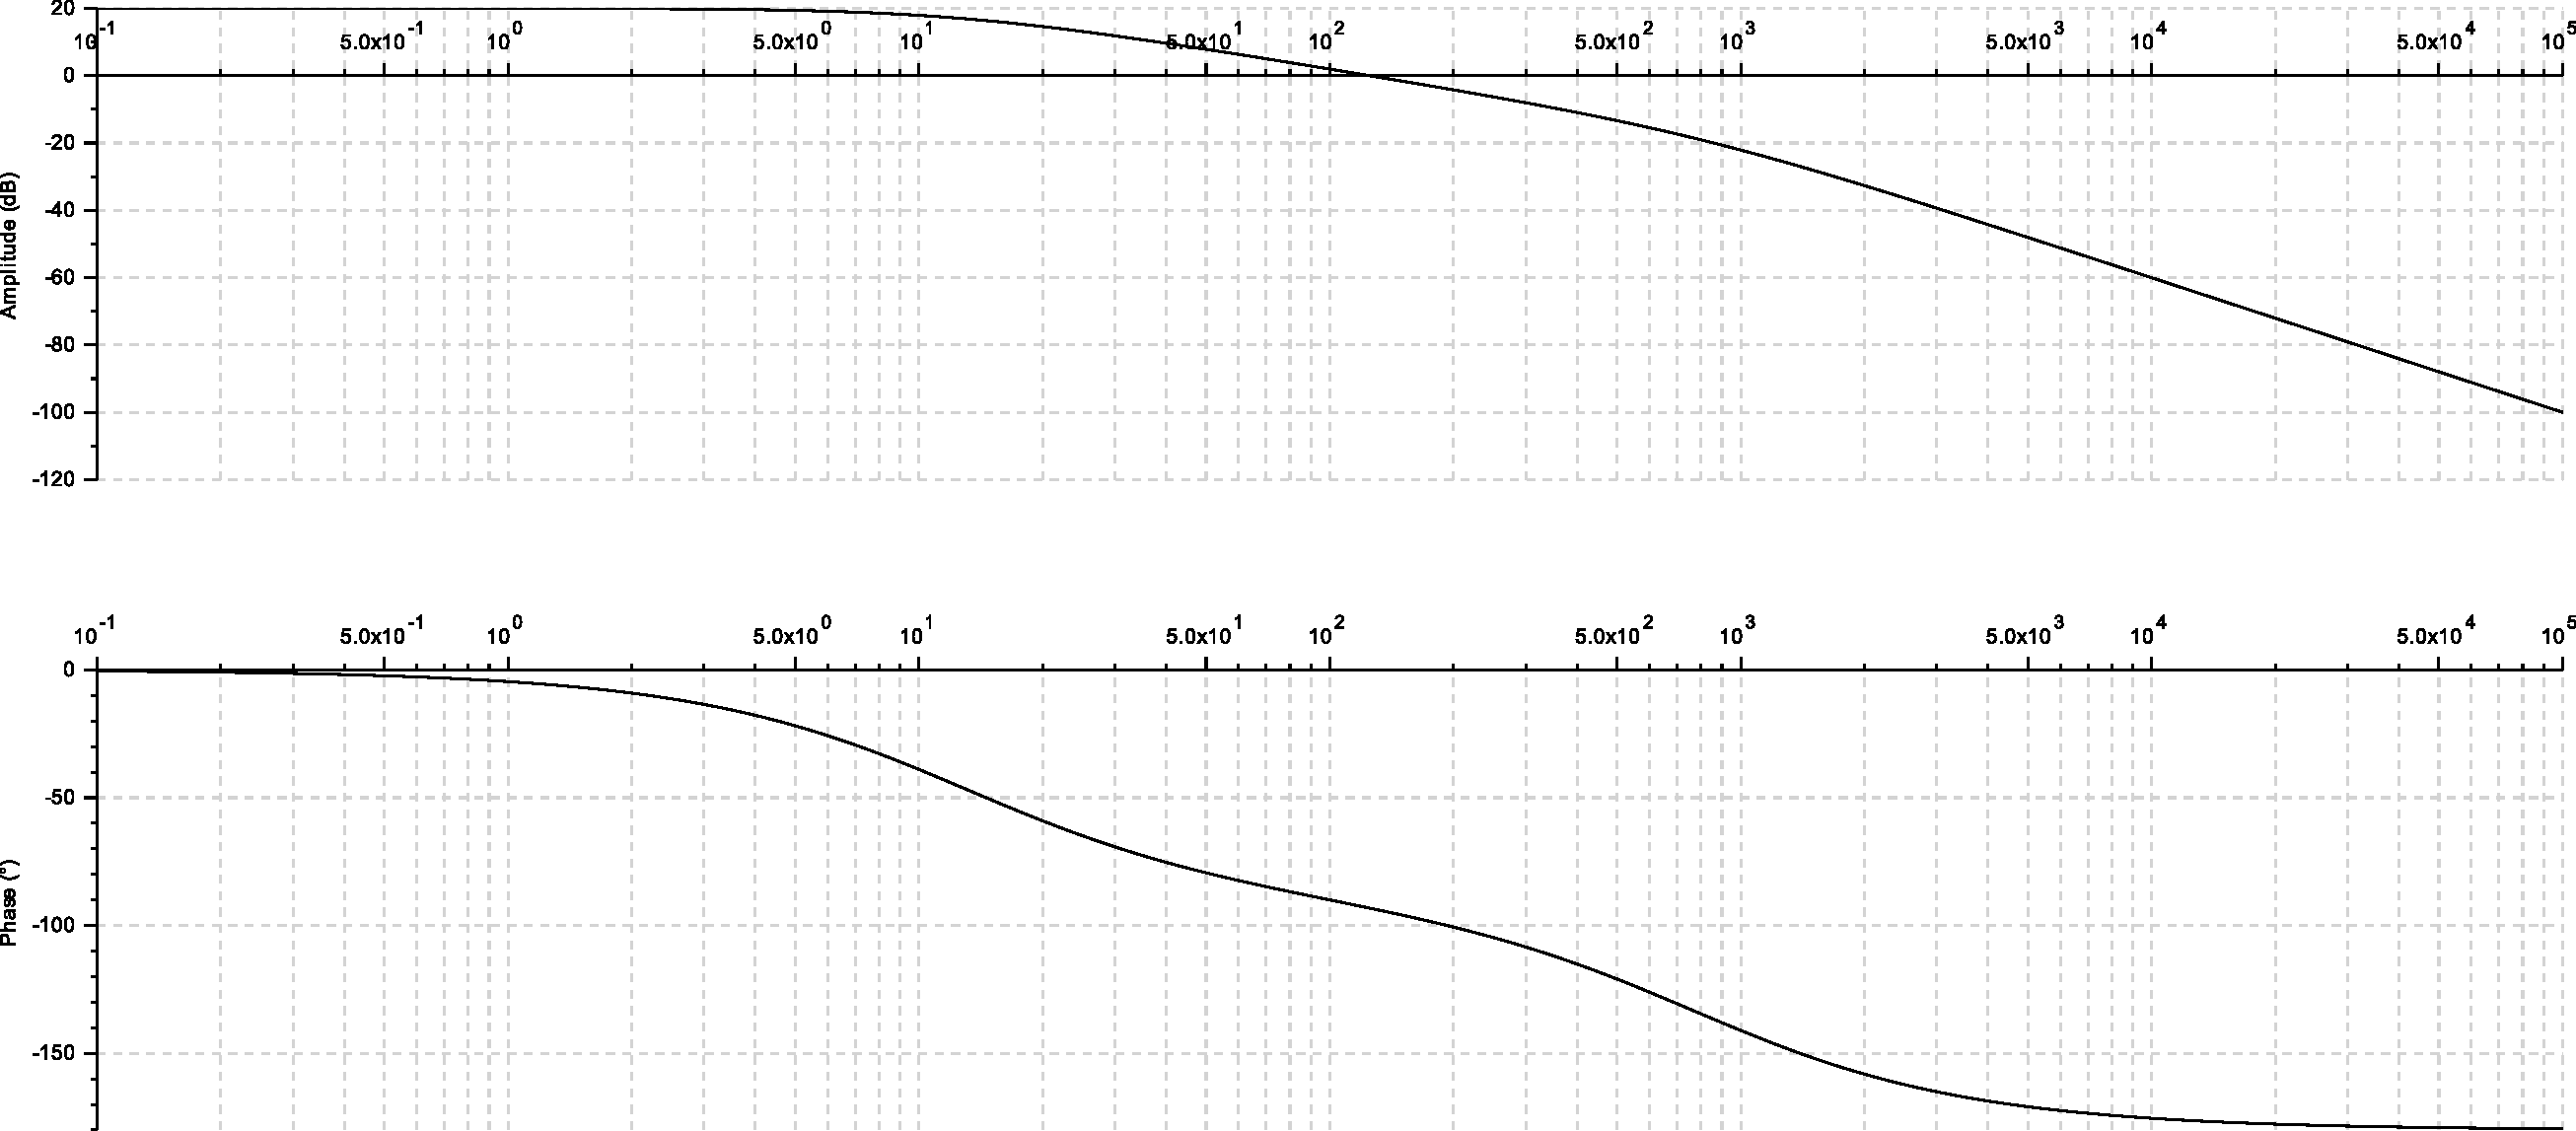
\includegraphics[width=0.9\linewidth]{img/BodeH1_cor}
\end{center}

\paragraph{Question 2:} Tracer les diagrammes de Bode de la fonction de transfert $H_2(p)$.

\begin{center}
$H_2(p)=\frac{40}{1+0,01.p+\frac{p^2}{90^2}}$
\end{center}

\begin{center}
 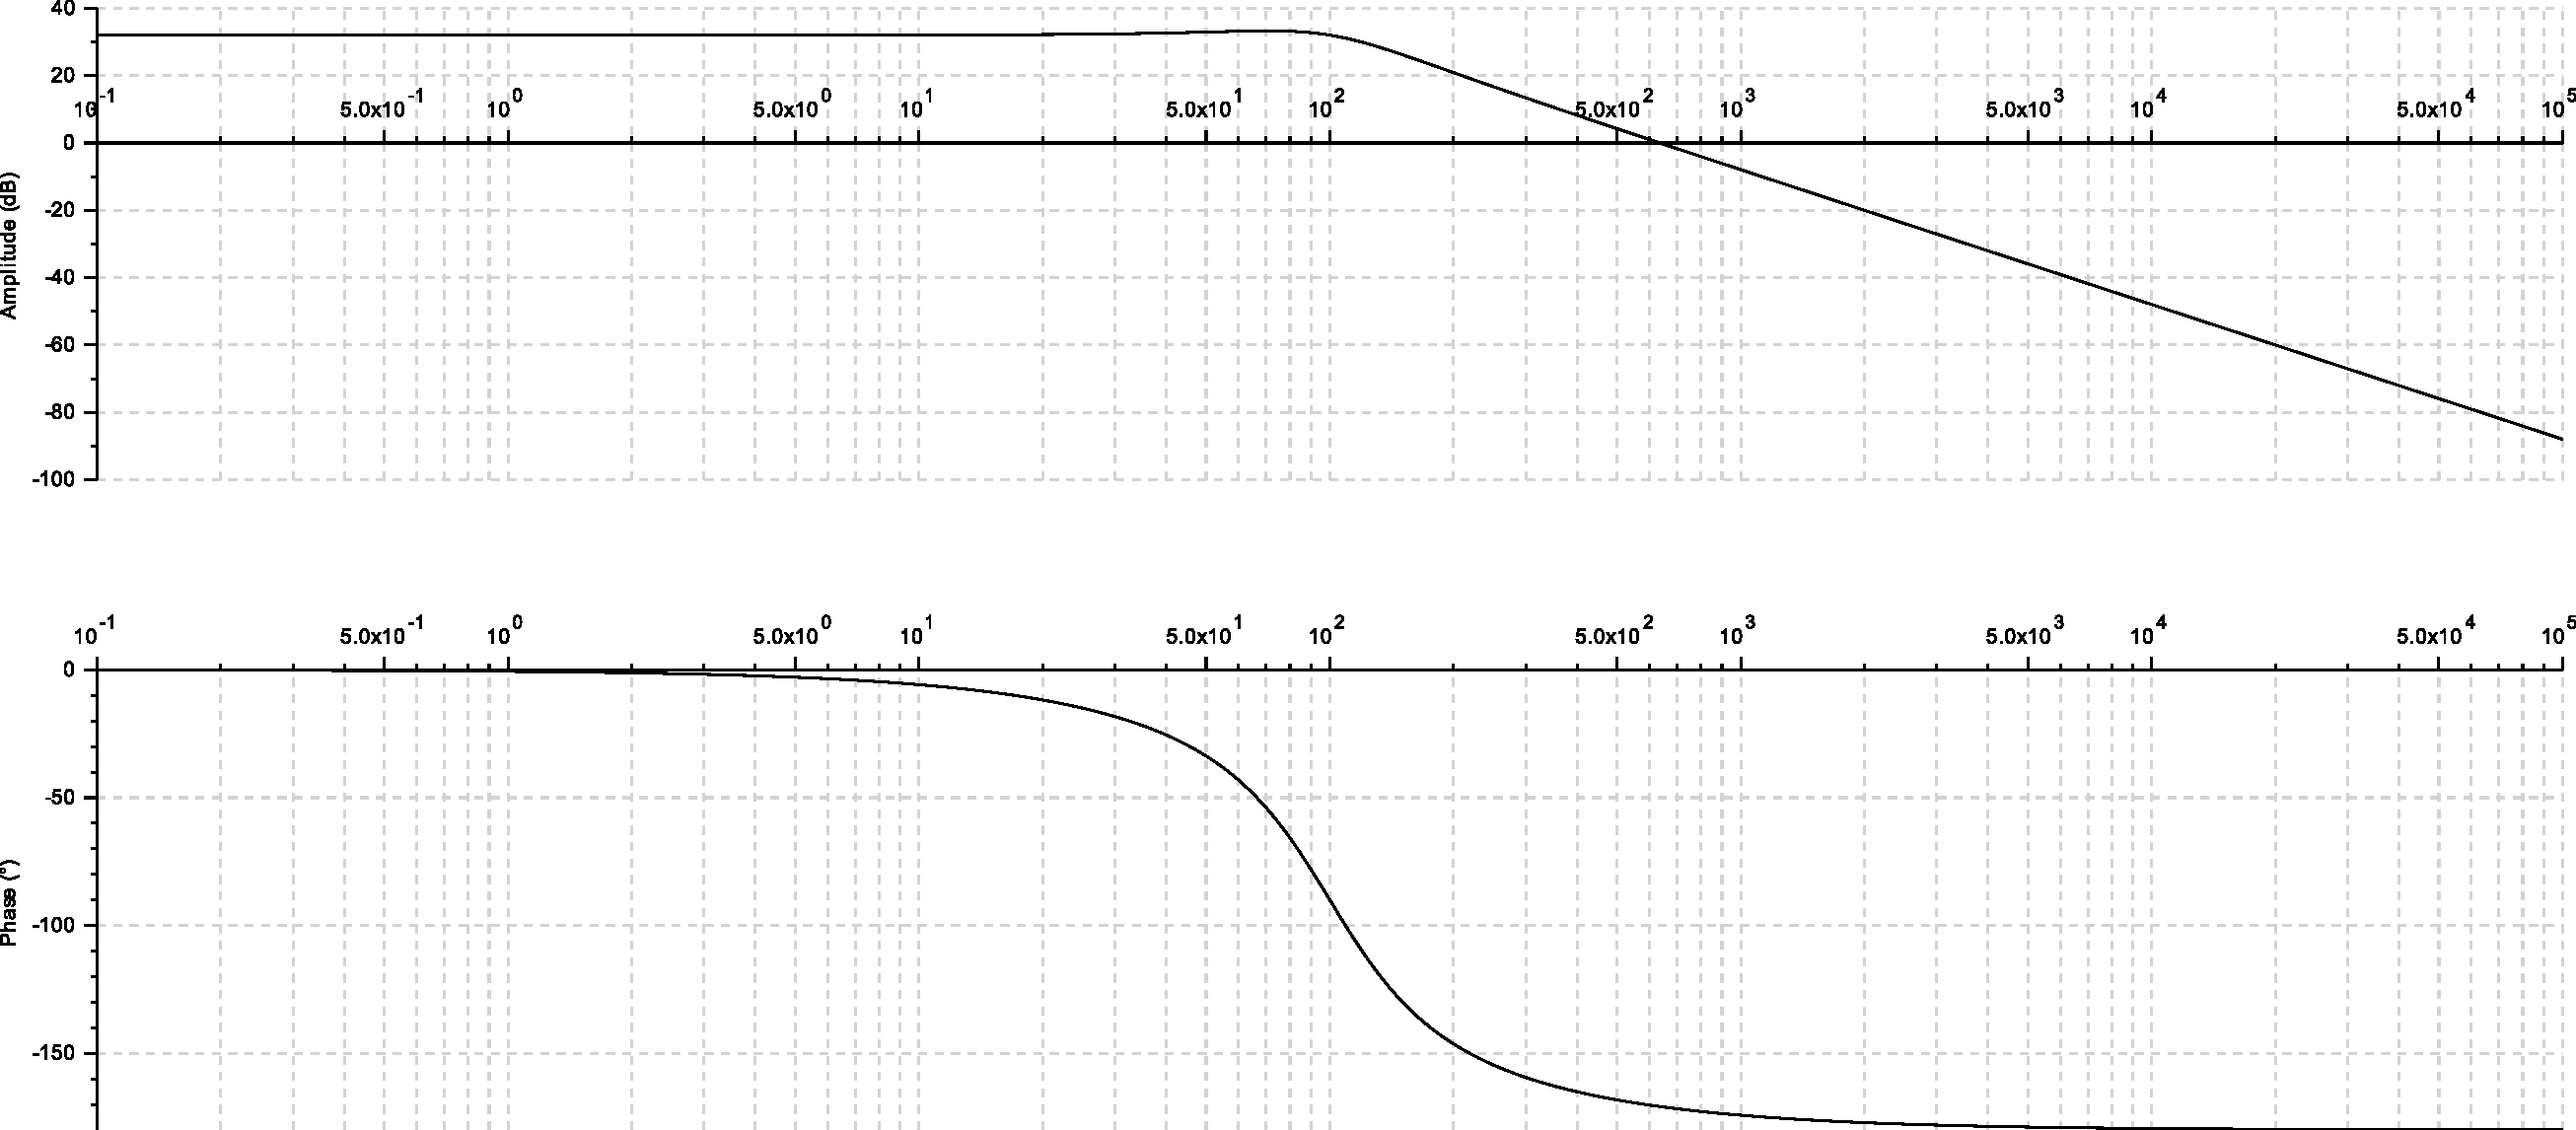
\includegraphics[width=0.9\linewidth]{img/BodeH2_cor}
\end{center}

\begin{center}
 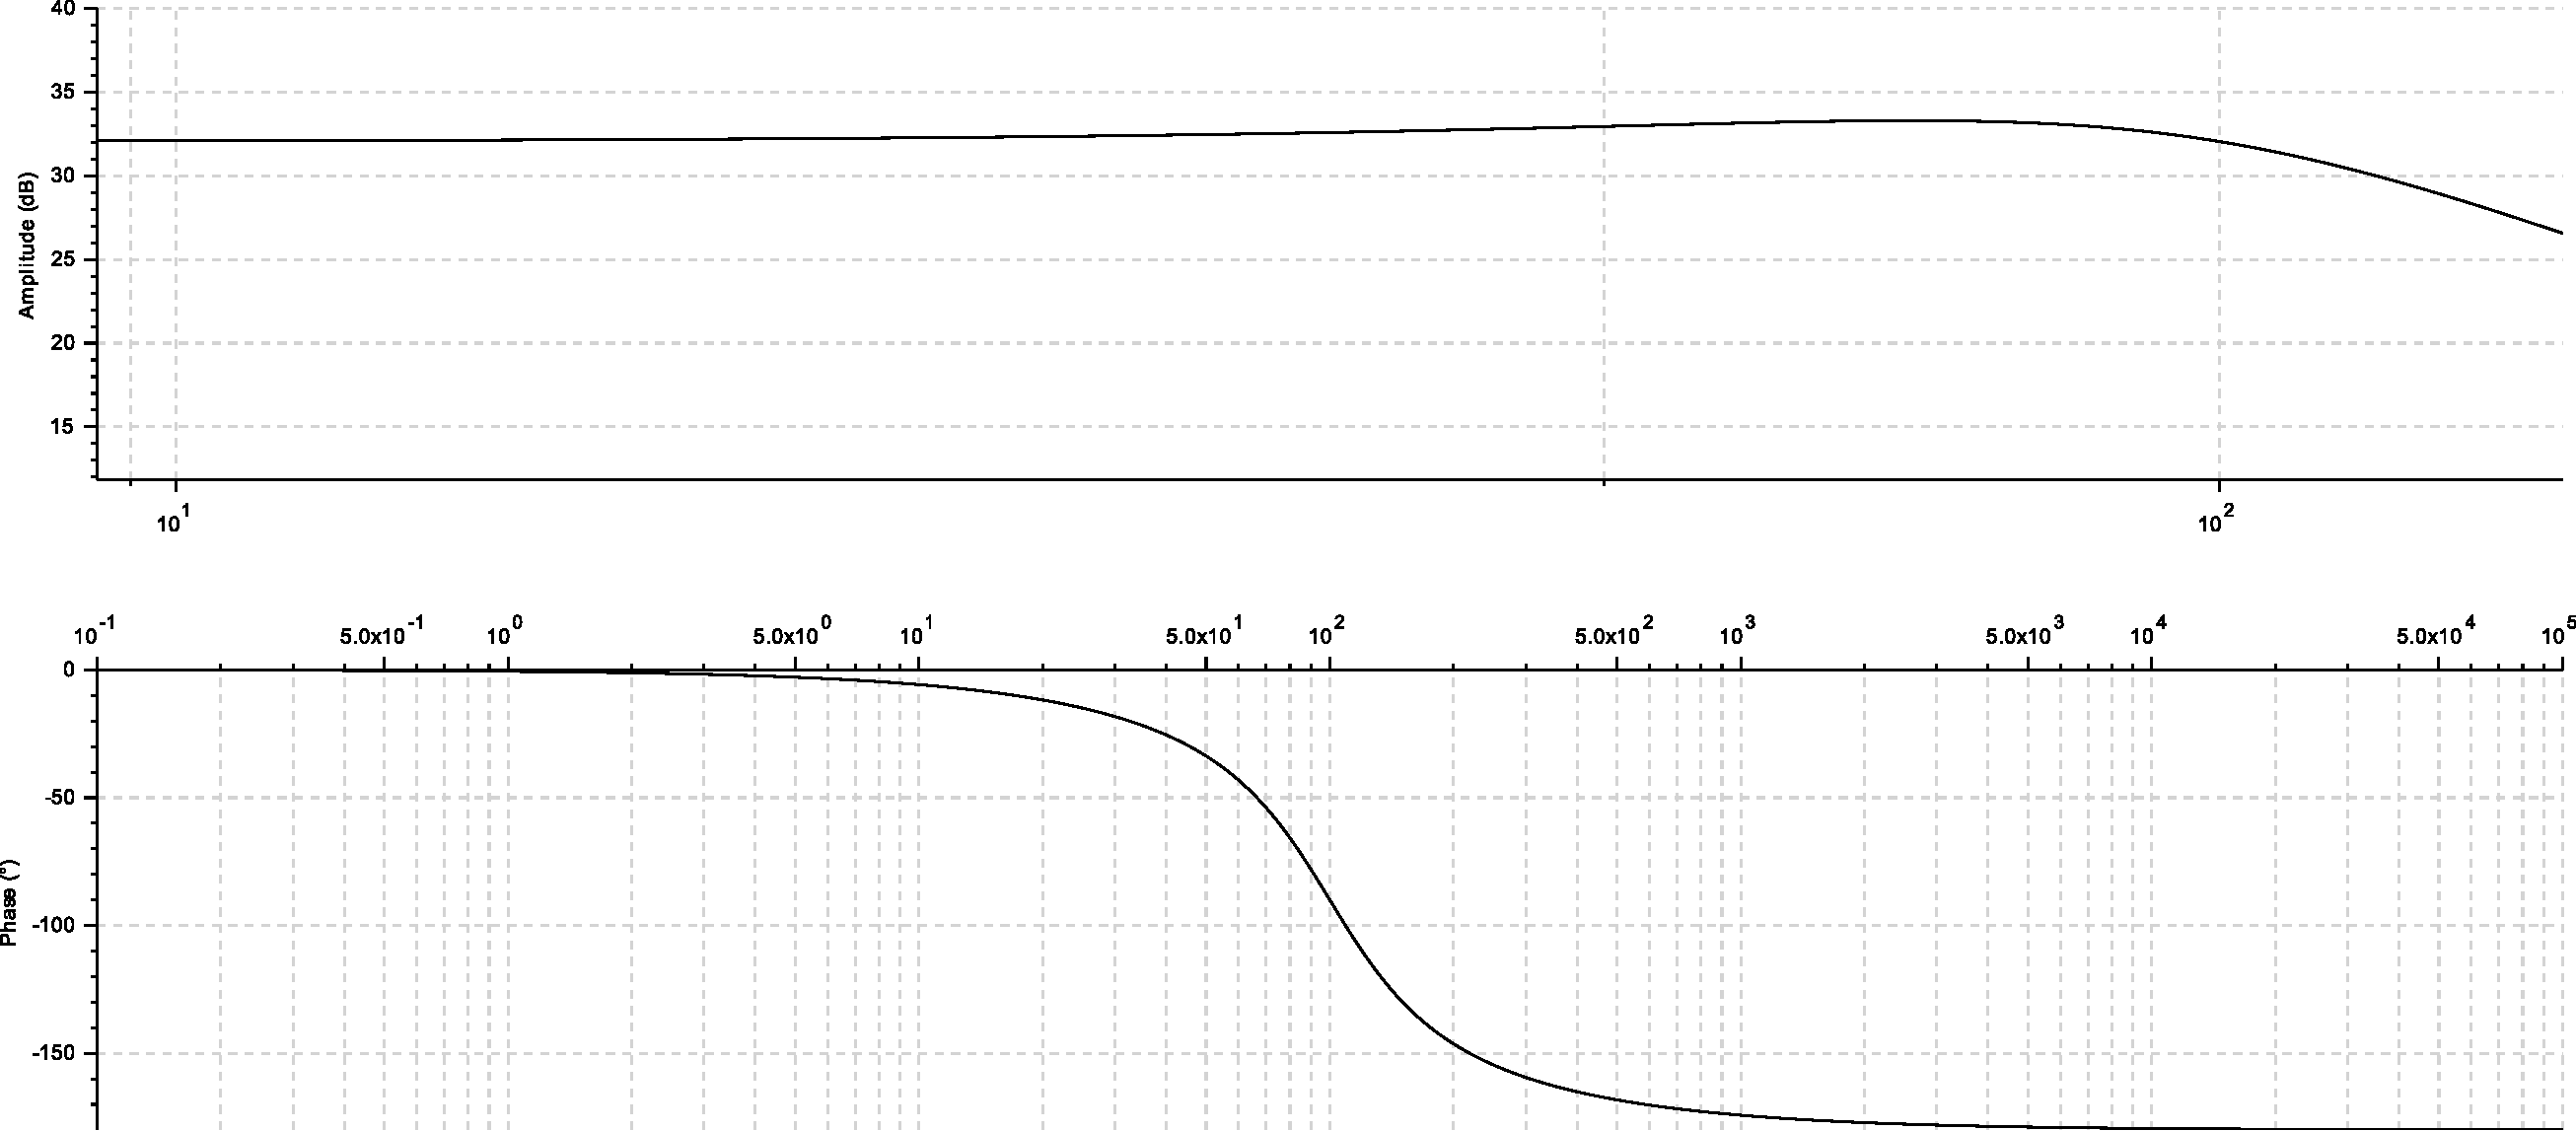
\includegraphics[width=0.9\linewidth]{img/BodeH3_cor}
\end{center}

\end{document}
